\documentclass[12pt,preprint]{aastex}
%\documentclass[preprint]{aastex}

\usepackage[textwidth=0.8in,colorinlistoftodos]{todonotes}
\usepackage[toc,page]{appendix}

%#For adding line numbers:
\usepackage{lineno}
\linenumbers


\usepackage{rotating}
\usepackage{amsmath}
\usepackage{graphicx}
\usepackage{xspace}
\usepackage{url}

% Note, hyperref has to come after other packages!
\usepackage{hyperref}

% some units
\newcommand{\kev}{\text{Kev}\xspace}
\newcommand{\mev}{\text{MeV}\xspace}
\newcommand{\gev}{\text{GeV}\xspace}
\newcommand{\tev}{\text{TeV}\xspace}
\newcommand{\sr}{\text{sr}\xspace}
\newcommand{\s}{\text{s}\xspace}
\newcommand{\ph}{\text{ph}\xspace}
\newcommand{\cm}{\text{cm}\xspace}
\renewcommand{\sec}{\text{s}\xspace}
\newcommand{\tsext}{{\ensuremath{\text{TS}_{\text{ext}}}}\xspace}
\newcommand{\tsinc}{\ensuremath{\text{TS}_{\text{inc}}}\xspace}
\newcommand{\loglikelihood}{\ensuremath{LL}\xspace}

\newcommand{\rsixeight}{{\ensuremath{\text{r}_{68}}}\xspace}

\newcommand{\tsextpointlike}{\ensuremath{\tsext_{,\pointlike}}\xspace}
\newcommand{\tsextgtlike}{\ensuremath{\tsext_{,\gtlike}}\xspace}

\newcommand{\ts}{\text{TS}\xspace}
\newcommand{\glon}{\text{GLON}\xspace}
\newcommand{\glat}{\text{GLAT}\xspace}
\newcommand{\altdiff}{\text{alt,diff}\xspace}
\newcommand{\altpsf}{\text{alt,psf}\xspace}
\newcommand{\sys}{\text{sys}\xspace}
\newcommand{\stat}{\text{stat}\xspace}

\renewcommand{\deg}{\ensuremath{^\circ}\xspace}

% the program names
\newcommand{\pointlike}{\text{\em pointlike}\xspace}
\newcommand{\python}{\text{\em python}\xspace}
\newcommand{\gtlike}{\text{\em gtlike}\xspace}
\newcommand{\gtobssim}{\text{\em gtobssim}\xspace}
\newcommand{\minuit}{\text{\em Minuit}\xspace}
\renewcommand{\approx}{\sim\!\xspace}

\shorttitle{Search for Extended LAT Sources}

\begin{document}

\title{Search for Spatially Extended Fermi-LAT Sources Using Two Years of Flight
Data}

\author{
J.~Lande\altaffilmark{3}, 
\altaffiltext{3}{W. W. Hansen Experimental Physics Laboratory, Kavli Institute for Particle Astrophysics and Cosmology, Department of Physics and SLAC National Accelerator Laboratory, Stanford University, Stanford, CA 94305, USA}
}


\begin{abstract}
We present a new method for analyzing 
the spatial extension of sources with
the Large Area Telescope (LAT), the primary science instrument on the
{\em Fermi Gamma-ray Space Telescope (Fermi)}. 
The source extension is an important input to correctly 
associate LAT sources with their counterparts at other
wavelengths. We provide
a series of Monte Carlo studies to validate this tool and calculate
the LAT's detection threshold to spatially extended sources.  We then
apply this tool to test all sources in the two year source catalog for
extension. We present on the detection of nine spatially extended sources
in addition to the twelve spatially extended sources reported in the
second Fermi-LAT Catalog (2FGL).
\end{abstract}

\listoftodos

\section{Introduction}

The Large Area Telescope (LAT) is a pair conversion telescope on the Fermi
Gamma-Ray Space Telescope (FGST). It has been surveying the $\gamma$-ray
sky since June 2008.  Fermi has a broad energy coverage (20 \mev to $>300$
\gev), wide field of view ($\approx 2.4 \sr$), and large effective area
($\approx 8000 \cm^2$ at $>1 \gev$).

Using two years of all sky surveying data, the LAT Collaboration
published a catalog of 1873 \gev sources\cite{second_cat}. Many of these can
be positionally associated with a variety of source classes including
Active Galactic Nuclei (AGN), pulsars, galaxies, and supernova
remnants (SNRs).  While many of the LAT sources can be
spatially
resolved when observed at other frequencies, detection of 
an extension at
\gev energies by the LAT is complicated by the rather large
point-spread function (PSF) of the instrument. The angular resolution
for events converting in the front part of the detector, defined as
the 68\% containment radius for a point source, is approximately
$3.5^{\circ}$ at 100 \mev, improving to about 0.1$^{\circ}$ at 10 \gev.

However, a number of sources positionally coincident
with LAT sources exhibit extension at other
wavelengths which are larger or comparable to the LAT PSF.
In particular certain SNRs, pulsar wind
nebulae (PWNe), molecular clouds, normal galaxies, 
galaxy clusters or dark
matter satellites can therefore be expected
to be observed as spatially extended sources in the LAT.
The LAT collaboration has previously reported on
the discovered of five spatially extended supernova remnants, IC443,
W28, W44, W51C, and RX J1713.7-3946
(\cite{ic443,w28,w44,w51c,rx_j1713_lat}). In addition, three extended
PWNe were detected: MSH 15-52, Vela~X, and
HESS\,J1825-137 (\cite{msh1552,velax,fermi_hess_j1825}), as well as
two close-by galaxies, the Large Magellanic and Small Magalenic Cloud
(\cite{lmc,smc}), and finally the radio galaxy Centarus A
(\cite{cen_a_lat}) .

For each of these sources, the extension was determined based on
dedicated analysis of the particular source or region of interest
instead of being the outcome of a systematic search of the LAT catalog.
For the systematic scan of all LAT catalog sources presented here, we
therefore expect to find additional spatially extended LAT sources, in
particular since many extended sources in the Galactic plane have been
detected at \tev energies using Air Cherenkov detectors and \tev and
\gev emission often originates from the same population of high-energy
particles.  A variety of spatially extended sources have been detected
in the Galactic plane at \tev energies. Most prominent was a survey of
the Galactic plane using the High Energy Stereoscopic System (H.E.S.S)
which presented 14 spatially extended sources
 with extensions varying from
$~0.1\deg$ to $~0.25\deg$ (\cite{hess_plane_survey}). In fact, within
our Galaxy only very few sources (most notably the $\gamma$-ray binaries
LS\,5039 (\cite{HESSLS5039}), LS I+61-303 (\cite{MAGICLSI, VERITASLSI})
and HESS\,J0632+057 (\cite{HESS0632}) are amongst the few Galactic sources
for which no significant extension was detected at \tev energies. Given
these findings, it can be expected that if the source population at \gev
energies has similar properties, that at least some of the Fermi-LAT
sources in our Galaxy should be spatially resolvable at \gev energies.

Being able to spatially resolve the \gev emission from a source is
important for several reasons. Because of the large PSF and the large
candidate source density in our Galaxy, source confusion is a severe
problem for the identification of LAT sources.  Finding a coherent
source extension across different energy bands allows a firm association
of a LAT source to an otherwise confused counterpart.  Because of the
strongly varying PSF of the LAT, the spatial and spectral information
about a source do not simply decouple. A biased spatial model will bias
the spectral model of the source. In particular, performing a spectral
analysis on a spatially extended source modeled as point-like will
systematically shift the spectral index to be softer.  Furthermore,
correctly modeling a source's extension is important for improving
the model of the sky and removing excess residuals, for example in the
region around surrounding the Large Magellanic Cloud (\cite{first_cat}).
Additionally, such excess residuals potentially bias the significance
and measured spectrum of neighboring sources in the densely populated
Galactic plane.

\section{Analysis Methods}

Morphological studies of sources in the \gev energy range using the
LAT are challenging because of the significantly energy-dependent PSF.
Additional complications arise close to the Galactic plane due to
systematic uncertainties in the Galactic diffuse emission.  The LAT's
PSF is limited at lower energies by multiple scattering in the tracker
and the 68\% containment radius of the PSF is approximately 5.1\deg
at 100 \mev  when averaged over instrument acceptance and including
photons which convert in either the thick or thin layers of the
tracker. The PSF improves with energy and approaches a limit given
by the granularity of the silicon strips and is 0.14\deg at 10 \gev
(\cite{on_orbit_calibration}).  The high resolution of the higher
energy photons in the LAT energy range however is offset by their low
statistics. Therefore a detailed investigation has been performed in this
work to determine the optimal energy range to measure source extension
(see below).

\subsection{The \pointlike Package}

A new analysis tool has been developed to address the unique requirements
for studying spatially extended sources with the LAT. The tool
provides a maximum likelihood analysis where the Poisson likelihood
for observing the measured counts is maximized,
given a parametrized spatial and spectral model of 
the source and its surrounding region.
The extension of a source can be modeled by a
geometric shape (e.g. a disk or Gaussian) and the source's position,
extension, and spectrum can be simultaneously fit.

This analysis is not feasible using the standard LAT likelihood
analysis tool \gtlike\footnote{\gtlike is distributed publicly by the
Fermi Science Support Center (\cite{fssc})} because \gtlike can only 
fit the spectral parameters of the model. 

We note that \gtlike has been used in the past in several studies of
source extension in the LAT collaboration (\cite{lmc,smc,w28,w51c}).
Based upon a set of \gtlike maximum likelihood fits at fixed extensions,
a profile of the likelihood as a function of the extension was calculated.
This approach is not optimal because the position, extension, and
spectrum of the source must be simultaneously fit to find the best fit
parameters and to correctly compute the statistical significance of the
detection.  Furthermore since the \gtlike likelihood profile approach
is computationally intensive, no large-scale Monte Carlo effort can be
run to validate it.

The approach presented here is based on a second maximum likelihood
fitting package developed in the LAT collaboration and called \pointlike
(\cite{first_cat,matthew_kerr_thesis}).  We extended the code to allow
a simultaneous fit of the source extension together with the position
and the spectral parameters.

The choice to base the spatial extension fitting on \pointlike
rather than \gtlike was made on considerations of computing time.
The \pointlike algorithm was optimized for speed to handle
larger numbers of sources efficiently which is important for
our catalog scan as well as the Monte Carlo validation of our method.
Details on the \pointlike package can be found in (\cite{matthew_kerr_thesis}).

\subsection{Extension Fitting}
\label{extension_fitting}

In \pointlike, it is assumed that the spatial and spectral model
of an extended source decouple and that the spatial shape can be
represented by a two dimensional function.  To fit the extended source,
\pointlike convolves the extended source shape with the PSF (as a
function of energy) and uses the \minuit fitting library to maximize
the likelihood by simultaneously fitting the position and extension
of the source (\cite{minuit_documentation}).  As will be described in
section~\ref{monte_carlo_validation}, simultaneously fitting the position
and extension is necessary to correctly calculate the statistical
significance of the detection of extension.  For each position and
extension, the spectral parameters of the sky model are refit. To avoid
projection effects, what is directly fit is not the longitude and latitude
but instead the source's displacement in a rotated reference frame.

The significance of the extension of a source can be calculated from
\tsext, which is defined as twice the increase in log likelihood (\loglikelihood)
between
the extended source model at its best fit values and the point source
model at its best fit values:
\begin{equation}
  \tsext=2\log(\loglikelihood_\text{ext}/\loglikelihood_\text{ps}).
\end{equation}
\pointlike calculates \tsext by fitting a source first with a spatially
extended model and then as a point source.  The interpretation
of \tsext in terms of a statistical significance is discussed in
section~\ref{monte_carlo_validation}.

The convolution of radially symmetric extended sources is optimized by
using a semi-analytic calculation.  The observed photon distribution
can be written as the convolution of the source shape ($I_\text{src}$)
with the PSF
\begin{equation}
  \text{PDF}(\vec r) = \int  \text{PSF}(|\vec r - \vec r'|)I_\text{src}(\vec r') d A'.
\end{equation}
For the LAT, the PSF is parameterized by a {\em King function}
\begin{equation}
  \text{PSF}(\vec r) = 
  \frac{1}{2\pi\sigma^2}
  \left(1-\frac{1}{\gamma}\right)
  \left(1+\frac{u}{\gamma}\right)^{-\gamma},
\end{equation}
where $\sigma$ and $\gamma$ are free parameters
(\cite{matthew_kerr_thesis}).  For radially symmetric extended sources,
the angular part of the integral can be done analytically
\begin{equation}
  \text{PDF}(u)= \int_0^\infty dv
  I_\text{src}(v) 
  \left(\frac{\gamma-1}{\gamma}\right)
  \left( \frac{\gamma}{\gamma + u + v}\right)^\gamma 
  \times ~_2F_1 \left(\gamma/2,\frac{1+\gamma}{2},1,\frac{4uv}{(\gamma+u+v)^2}\right).
\end{equation}
This convolution formula is used by \pointlike because it is faster
and more closely reduces to the PSF when the source's size is 
small.

There will always be a small numerical discrepancy between the PSF and
a very small extended source due to numerical error in the convolution.
In most situations, this error would be insignificant. But when testing
a source for extension, this offset can significantly bias the estimate
of the significance of the extension of a source.  To correct for this,
when testing a source for extension we compare the likelihood fitting
the source with an extended shape to the likelihood fitting it with its
extension fixed to ${10^{-10}}\deg$.

\subsection{Extension Errors}
\label{extension_error}

Errors on fit parameters are typically calculated in one of two
ways. The first method requires explicitly varying a parameter
while simultaneously optimizing the other parameters
until the log of the likelihood has fallen by a particular value.
The \minuit fitting
package provides the {\em Simplex} function to calculate errors this way
(\cite{minuit_documentation}).  The second method involves estimating the
likelihood function as being a multivariate Gaussian and calculating the
curvature of the log of the likelihood at the peak to estimate when the
function will decrease by the desired value. \minuit provides the {\em HESSE}
algorithm to calculate errors this way.  {\em HESSE} errors 
can be calculated significantly faster.

We found that the {\em HESSE} errors on the extension of a source
were sometimes badly estimated.  On the other hand, the {\em Simplex}
algorithm was prohibitively slow and would often fail to convergence. Our
approach to calculating extension errors is to fix the position of the
source and varying just the extension using the {\em Simplex} algorithm.
This approach makes the approximation that the covariance between each
spatial parameter is small but not that the likelihood is Gaussian. This
method is shown schematically in figure~\ref{four_plots_ic443}(a) which
shows the change in \loglikelihood when varying the extension of the
SNR IC443.  The localization error is separately calculated by fixing
the extension and spectrum of the source and fitting a parabola to the
likelihood as a function of position.

\subsection{\gtlike Crosscheck}
\label{gtlike_crosscheck}

\pointlike is important for LAT analysis that require many iterations
such as source localization and extension fitting.  On the other hand,
because of the fewer approximations used in calculating the likelihood
we expect that the spectral parameters fit by \gtlike to be slightly
more precise.  Furthermore, because \gtlike is the standard likelihood
analysis package, it has been more extensively validated for spectral
analysis.  For that reason, in the following analysis  we use \pointlike
to determinate the position and extension of a source and then determine
the spectrum using \gtlike. Both \gtlike and \pointlike can estimate
the statistical significance of the extension of a source and we require
that both methods agree to claim a detection.

We found good agreement between the two methods. For the new extended
source candidates, table~\ref{alt_diff_model_results} will shows a
comparison of \ts and \tsext computed using \pointlike and \gtlike.
Unless explicitly mentioned, all \ts, \tsext, and spectral parameters
were calculated using \gtlike using \pointlike's positions and extensions.

\subsection{Dual Localization}
\label{dual_localization_method}

There is a degeneracy between a spatially extended source and multiple
point sources.  To assess the possibility of source confusion,
we developed a function in \pointlike to simultaneously fit the position
of two point sources.  To improve the robustness of the fit, the sum and
difference of the positions of the two sources are fit in a coordinates
rotated to the equator.  The \loglikelihood is then maximized by fitting
the sum and difference of the positions.

We define \tsinc as twice the increase in \loglikelihood fitting the
region as two point sources compared to fitting the region as one point
source: \begin{equation}
  \tsinc=2\times(\loglikelihood_\text{2pts}-\loglikelihood_\text{ps}).
\end{equation} \tsinc can not be directly compared to \tsext to see
which model is more significant because the models are not nested
(\cite{statistics_with_care}). Even though the comparison of \tsext
with \tsinc is not a calibrated test, we find the extreme cases $\tsinc
\loglikelihood \tsext$ or $\tsinc\gg\tsext$ to be suggestive and we only
consider a source to be extended if $\tsext>\tsinc$.

Like extended sources described in section~\ref{gtlike_crosscheck},
the spectrum of the two point sources can be refit using \gtlike.
we quote the spectral values obtained from \gtlike using the best fit
positions found using \pointlike.  For the extended candidates found
by our search, we computed both \tsext and \tsinc.  The results will be
presented in table~\ref{dual_localization_results}.

\subsection{Comparing Source Sizes}

\label{compare_source_size}

The spatial shape of extended sources can be modeled
as a two dimensional Gaussian
\begin{equation}\label{gauss_pdf}
  \text{PDF}(x,y)=\tfrac{1}{2\pi\sigma^2}\exp\left(-(x^2+y^2)/2\sigma^2\right)
\end{equation}
or a uniform disk
\begin{equation}\label{disk_pdf}
  \text{PDF}(x,y)=\tfrac{1}{\pi\sigma^2}\delta\left(x^2+y^2<\sigma^2\right).
\end{equation}
Although these shapes are significantly different, the convolution of them
with the PSF look similar.  Figure~\ref{compare_disk_gauss} demonstrates
this by showing the PSF, PDF, and convolution of the PDF with the PSF
for a uniform disk and Gaussian spatial model of size 0.5\deg.  This plot
shows that we are not very sensitive to probing the exact structure of an
extended source.  In the following we assume a uniform disk spatial model.

To get the convolved shapes to match in figure~\ref{compare_disk_gauss},
we had to set them to predict the same 68\% containment
radius of 0.5\deg.  The 68\% containment radius for a
spatial model is the radius at which 68\% of the intensity is
enclosed.  It can be computed by a straightforward integral
and we find that $\rsixeight_\text{,Gaussian}=1.51\sigma$
whereas $\rsixeight_\text{,disk}=0.82\sigma$ where $\sigma$
is defined in equation~\ref{disk_pdf} for the Gaussian source and
equation~\ref{gauss_pdf} for the disk source.  Since $\rsixeight=0.5\deg$,
the uniform disk has $\sigma=0.41\deg$ and the Gaussian has
$\sigma=0.75\deg$.

This is important when comparing morphologies to other wavelengths
because the quoted size can vary significantly depending on which quantity
is reported.  This effect can be best seen in figure~\ref{compare_r68}
which a counts map of an extended source simulated in the energy
range from 1 \gev to 100 \gev with a uniform disk spatial model with
an extension $\sigma$ of 0.5. Overlaid on the plot is the fit extension
assuming the source has a uniform disk and a Gaussian spatial model. The
plot overlays both $\sigma$ and $\rsixeight$ and $\sigma$ is significantly
larger for the disk spatial hypothesis compared to the Gaussian spatial
model. On the other hand, the disk and Gaussian's 68\% containment radius
are similar.

Since we are not very sensitive to the particular morphology of an
extended source, there is no correct choice for which size to quote
or which shape to overlay. For the following analysis, we quote the
disk's edge and overlay this size.  But due to smearing of the PSF,
$\sigma$ typically looks larger than the observed counts distribution.
When comparing the fit extensions with other wavelengths, it is important
to compare consistent quantities.


\section{LAT Extended Source Validation}


\subsection{Significance of Extension}
\label{monte_carlo_validation}

We validated \pointlike's extension fitting code with a Monte Carlo
study. \tsext (defined in section~\ref{extension_fitting}) can be used to calculate the statistical significance
of the extension of a source.  Since the point source and extended source models are
nested, an extended source must always fit as well as a point source.  On the other hand, we would
not expect the likelihood to change very much unless the source was
significantly extended.  Since an extended source has one additional
degree of freedom, Wilks' Theorem predicts that the distribution of $\tsext$
when testing a point source for extension should follow a $\chi^2_1$
distribution (\cite{wilks_theorem}).

However, since the null hypothesis rests on the edge of
parameter space when the extension is 0, Wilks' Theorem does not hold
(\cite{warn_wilks_theorem}).  One might expect the actual distribution
to be a half $\chi^2_1$ distribution with one degree of freedom plus
half a delta function at 0:
\begin{equation}
  P(\ts)=\tfrac{1}{2}(\chi^2_1(\ts)+\delta(\ts)).
\end{equation}
Chernoff proved that under certain assumptions this is the correct distribution
when the null hypothesis is on the edge of parameter
space (\cite{chernoff}).  The false detection
probability can be estimated by integrating this function from an observed
test statistic value to infinity. It is for this particular distribution
that the often quoted result holds that $\sqrt{\ts}$ is a measure of
the number of $\sigma$ of the detection (\cite{mattox_egret}).

The half $\chi^2_1$ distribution was found to hold for the special case
of source finding using EGRET (\cite{mattox_egret}). This distribution
is also plausible when testing point sources for extension. Due to
statistical fluctuations, half of the point sources might look narrower
than the PSF leading to $\tsext=0$. The other half of the time, we would
get a distribution consistent with Wilks' theorem. We will present a
Monte Carlo study that shows an empirical distribution of \tsext in the
null hypothesis and compares it to this distribution.

We simulated point sources of varying spectral models and fit them
them using \pointlike as both point and extended sources. The data was
simulated using \gtobssim\footnote{\gtobssim is distributed
by the Fermi Science Support Center (\cite{fssc}).}
The point sources were simulated with a power-law spectral model with
six $>100$ \mev fluxes ranging from $3\times 10^{-9} \ph/\cm^2/\sec$ to
$10^{-6} \ph/\cm^2/\sec$.  The point sources were simulated with spectral
indices ($\gamma$) of 1.5, 2, 2.5, and 3.  These values were picked to
to represent typical source parameters in LAT-detected sources. The point
sources were simulated on top of an isotropic power-law background
with a Sreekumar-like spectrum ($>100$ \mev flux of $1.5\times 10^{-5}$ and spectral
index 2.1) (\cite{sreekumar_isotropic}).  The Monte Carlo simulation was
performed over a one year time interval using a default rocking profile
and a representative livetime fraction of 0.8.  The reconstruction was
performed with photons from an energy range of 1 \gev to 100 \gev using 4
energy bins per decade and using the 
Pass 7\_V6 (P7\_V6) Source Instrument
Response Function (IRFs).  For each point source, we used \pointlike
to fit it as both a point and extended source and calculate \tsext and
we only kept the sources which had a significant point source detection
($\ts>25$).


For most of the spectral models, ~30,000 statistically independent
simulations were performed. For the dimmer spectral models, many of the
simulations had $\ts<25$ and were discarded.  Table~\ref{ts_ext_num_sims}
shows the different spectral models used in our study as well as the
number of simulations.  The cumulative density of \tsext is plotted in
figure~\ref{ts_ext_mc}. The $\chi^2_1/2$ distribution suggested by Wilks'
Theorem is overlaid for comparison.

Our Monte Carlo study shows broad agreement between simulations and Wilks'
theorem. Nevertheless, the agreement is not perfect.  It should be noted
that the discrepancy seems to be worst for bright sources which seems to
imply that numerical errors in the convolution become more apparent for
sufficiently bright sources.  Other possible reasons for departure from
Wilks' theorem might include \pointlike ignoring energy dispersion which
would change the PSF's shape as a function of energy. But we emphasize
that most of the time, our empirical curve lies to the left of the
theoretical curve so using the theoretical distribution would lead to an
underestimate of the statistical significance of a detection. Therefore,
we are confident that $\sqrt{\tsext}$ can be used as a measure of the
statistical significance of a source's extension and use it in the
following analysis.

\section{Extended Source Detection Threshold}\label{extension_sensitivity}

We calculated the LAT's detection threshold to spatially
extended sources. The detection threshold to extension is
defined as the flux at which the average value of $\tsext$ is
$\langle\tsext\rangle=16$ corresponding to a $4\sigma$ detection (see
section~\ref{monte_carlo_validation}).  Qualitatively, we expect the LAT
would not be sensitive to sources much smaller than the PSF or much larger
than the PSF.  Small sources would look too much like the PSF and larger
sources would get lost in the background due to low surface brightness.

To calculate the LAT's detection threshold, we simulated sources with
a uniform radially symmetric disk spatial model on top of a power-law
Sreekumar-like isotropic spectrum (\cite{sreekumar_isotropic}).  The Monte
Carlo simulation was performed using the same two year time range that
was used in 2FGL.  For each extension and spectral index, we picked a
flux range which bracketed $\tsext=16$. We then picked ten flux points in
this range and repeatedly simulated and then performed extension tests of
the simulated extended source.  We calculated $\langle\tsext\rangle=16$
by fitting a line to the flux and $\tsext$ values.

Figure~\ref{index_sensitivity} shows the threshold for sources of four
spectral indices from 1.5 to 3 and extension varying from $\sigma=0.1\deg$
to $2.0\deg$.  The LAT's threshold to extension
is better for harder sources with more high energy photons and
the threshold is best for sources with an extension 
$\approx0.5\deg$ and is significantly worse for very small extended small.
Figure~\ref{index_sensitivity} shows the threshold using photons with
energies between 100 \mev and 100 \gev and also using only photons
with energies between 1 \gev and 100 \gev.  Except for the hardest
and largest sources, our detection threshold is almost unchanged when
including photons with energies between 100 \mev and 1 \gev.  This is also
demonstrated in figure~\ref{four_plots_ic443}(b) which shows \tsext for the
SNR IC443 computed independently in twelve energy bins between 100 \mev and
100 \gev. For IC443, which has a spectral index $\approx2.4$, almost the entire
increase in \ts comes from energies above 1 \gev.  On the other hand,
other systematic errors become increasingly important at low energy. For
our extension search, we use only only photons with energy above 1 \gev.

Figure~\ref{diff_factor_sensitivity} shows how the LAT's detection
threshold increases with increasing background. We compute the threshold
using 1, 10, and 100 times the Sreekumar-like isotropic background. The
latter factor approximately represents the intensity of the Galactic
diffuse emission near the Galactic center.  The figure shows the threshold
using only photons with energies between 1 \gev and 100 \gev and aldo
when using only photons with energies between 10 \gev and 100 \gev. We
are less sensitive to extended sources with higher background. Also,
given the same flux we are more sensitive to the source if those
photons have a higher energies.

Overlaid on figure~\ref{diff_factor_sensitivity} are the LAT
detected extended sources from table~\ref{known_extended_sources} and
table~\ref{new_ext_srcs_table}.  The extended sources are color coded
based upon whether the galactic diffuse and isotropic emission model is
closer to 1, 10, or 100 times the Sreekumar-like isotropic spectrum.

Finally, figure~\ref{all_sensitivity} shows the LAT's detection threshold
for all four spectral indices (1.5, 2, 2.5, and 3) against all three
background levels (1, 10, and 100 times the Sreekumar-like isotropic
background).  For a fixed 1 \gev to 100 \gev or 10 \gev to 100 \gev
flux, the LAT's detection threshold is only weakly depends upon the
spectral index.  This effect is most pronounced when using only photons
with energies above 10 \gev. The extension thresholds are tabulated in
table~\ref{all_sensitivity_table}.

\section{Extended Source Search Method}

2FGL is a list of 1873 \gev sources detected by the LAT.  2FGL included
twelve previously published spatially extended sources but did not
attempt to fit the extension of these sources. Other than these sources,
all 2FGL sources were modeled as point sources and 2FGL did not attempt to
resolve the extension of new sources.  In this paper, we tested all 2FGL
sources for extension to search for new spatially extended \gev sources.

For this search, we build a model of the
sky consistent with 2FGL.   We used the same two
years of data from August 4, 2008 to August 1, 2010 and we used the same
Pass 7\_V6 (P7\_V6) Source class event selections and 
Instrument Response Functions (IRFs, \cite{lat_on_orbit_psf}).  We used the same Galactic diffuse,
isotropic diffuse, and earth limb emission model. The spectrum of the
Galactic and isotropic diffuse models were refit during the analysis
while the earth limb emission was fixed to it's predicted value.

As was shown, we gain little in sensitivity using photons with energies
below 1 \gev. On the other hand, the large PSF at low energy makes us
more susceptible to systematic errors arising from source confusion due
to multiple point sources and susceptible to incorrect modeling of the
Galactic diffuse emission. In addition, the Galactic diffuse emission
is more pronounced at lower energies due to its steep energy spectrum.
For that reason, we performed our search using photons only between 1
\gev and 100 \gev.  We used 4 energy bins per each logarithmic decade
in energy.

We also performed a search for extended sources using photons only
between 10 \gev and 100 \gev. Even though we are testing the same
sources, this approach is complimentary because the Galactic diffuse
emission is even less dominant above 10 \gev. Furthermore, source
confusion becomes less of a problem since most LAT sources are not
significant at energies above 10 \gev.  Using higher energies, we might
expect to detect harder sources in more complicated regions. This is
beneficial for regions near pulsars which cutoff before 10 \gev and was
successfully used in detecting HESS\,J1825-137 and MSH 15-52 with the LAT
(\cite{msh1552,fermi_hess_j1825}).

For each catalog source, we tested it for extension using \pointlike
assuming the source had a uniform radially symmetric disk spatial model.
We used a circular $10\deg$ region of interest centered on our source and
included all catalog sources within $15\deg$ of the source of interest.
We refit the spectral parameters of sources within $2\deg$ of the source.
We modeled each source with a power-law spectral model. This was reasonable because for a source to be significantly
extended, it would have to be fairly hard and fit reasonably well by
a power-law. Second, since we began the analysis at either 1 \gev or
10 \gev, we didn't expect there to be significant curvature over this
energy range.

Finally, when analyzing the region, we automatically removed other
2FGL sources which were within 0.5\deg of the source of interest. This was done because of
a concern that extended sources would end up 2FGL as
multiple point sources. These spurious sources would then
distort the extension fit.
For each extended candidate, we performed a dual localization procedure
(described in section~\ref{dual_localization_method} to test if the
source is extended. We select the sources where $\tsext>16$.

\subsection{Additional Analysis}

Since extragalactic sources are typically too far away to be resolvable,
we expect most extended sources to be inside our Galaxy and most
likely on the Galactic plane.  Unfortunately, the \gev emission
in the Galactic plane is dominated by extremely structured Galactic
diffuse emission.  Finding sources on top of this emission is difficult
(\cite{first_diffuse_paper}) as has been discussed in 1FGL and 2FGL
(\cite{first_cat,second_cat}).  Furthermore, the Galactic plane is crowded
and it is often difficult to correctly model nearby sources.  Because of this,
finding a source with $\tsext>16$ is not a sufficient
criteria for resolving a source. For each extended source,
we perform several analysis crosschecks.

% 2FGL J1856.2+0450c = P72Y3047 for
As an example of why this is important, we describe the test of 
2FGL\,J1856.2+0450c for extension.  Figure~\ref{example_bad_fit} shows
a Galactic and isotropic diffuse emission subtracted
smoothed counts map of this source using photons with energy 
between 1 \gev and 100 \gev. 
In this region along the Galactic plane, there appears to be 
large-scale residual in the diffuse emission. As a result, 2FGL\,J1856.2+0450c 
fit to an extension of 1.83\deg and the result is statistically significant
with \tsext=45.4.  By looking at the residuals, it is clear that this
complicated region is not fit well even though the source's extension is
statistically significant. For this reason, we manually discard
the extension of this and similar sources.
% information came from
% /nfs/slac/g/ki/ki03/lande/extended_catalog/2FGL/v15/standard_analysis/spectral_emin_1000_v1/P72Y3047/v1/results_followup_P72Y3047.yaml

For each extended source candidate,
we took the spatial and spectral model found using \pointlike and
performed a crosscheck by refitting the spectral parameters using
\gtlike.  We used a square ROI $14.1\deg$ in diameter with $1/32\deg$
spatial bins and the same energy binning as \pointlike. Using \gtlike,
we found a second measure of \tsext, this time not fitting the extension
but using a fixed template with the extension determined by \pointlike.
We only considered a source to be significantly extended if \pointlike
and \gtlike both agreed.  For the new extended source candidates,
table~\ref{alt_diff_model_results} will show a comparison of of \tsext for
\gtlike and \pointlike.

For each candidate, we generated a map of residual \ts
by adding a new source of spectral index 2 into the region and finding
the increase in likelihood when fitting its flux. \ts maps are useful
to look for residual structure in the sky mode.  Figure~\ref{res_tsmaps}
shows a residual \ts map for the extended source IC443.

For each candidate, we generated plots of the sum of all counts
within a given distance of the source and compared it to the model
predictions of a point source.  The plots were binned uniformly
in $\Delta \theta^2$ so that an isotropic background would be flat.
An example radial integral plot is shown for the extended source IC443
in figure~\ref{four_plots_ic443}(c).  For each source, we also made
Galactic and extragalactic diffuse emission subtracted smoothed counts
maps. Figure~\ref{four_plots_ic443}(d) shows an example for IC443. 

For each source, we tested to see if the region contained instead
multiple point sources by replacing the extended source with
two point sources and performed the dual localization procedure
described in section~\ref{dual_localization_method}.  We only
considered a source to be extended if $\tsext>\tsinc$.  For the new
extended sources, we will show the results of this dual localization in
table~\ref{dual_localization_results}.

Because of the high source density in the Galactic plane, for promising
candidates we often had to iteratively improve the model of our background
sources to obtain a better fit of the sources.  Often, several catalog
sources would fill in the emission of the extended source and would
have to be removed from the region.  Similarly, background sources
were often insignificant in the fit energy range and had to be removed.
The position of background sources would often have to be refit once the
extended source was fit.  When the model of the extended source coupled
strongly with nearby sources, we iteratively fit the extended source and
all nearby sources until the fit converged.  For each extended source,
we describe the modification that were required.

\subsection{Systematic Errors on Extension}
\label{systematic_errors_on_extension}

% Alternative PSF

We estimate a systematic error on the extension of a source due to
uncertainty in our knowledge of the angular resolution of the LAT.  Before
launch, the LAT PSF was determined by a detector simulation which was
verified in accelerator tests (\cite{atwood_LAT_mission}).  A discrepancy
was found in flight data above a few \gev in the PSF compared to the
shape of bright AGN.  A publication on this issue is in preparation
(\cite{lat_on_orbit_psf}).  Subsequently, the PSF was fit empirically to
bright AGN and this empirical parameterization is the default PSF used
in the P7\_V6 IRFs.  To account for this uncertainty in our knowledge of
the PSF, we refit our extended source candidates using the Monte Carlo
representation of the PSF and consider the difference in extension found
using the two PSFs as a systematic error on the extension of a source.
Because the Monte Carlo representation of the PSF is smaller, it leads
to unphysically higher \tsext values.  This same approach was used in
(\cite{ic443}).  At high energies, we believe that our parameterization
of the PSF from bright AGN is substantially better than the Monte Carlo
representation of the PSF so this systematic errors is conservative.

% Alternate Diffuse

We estimate a second systematic error on the extension of a source
due to uncertainty in the model of the Galactic diffuse emission by
using an alternative diffuse model. The alternative model was based on
the GALPROP\footnote{GALPROP is a software package for calculating the
Galactic $\gamma$-ray emission based on a model of cosmic-ray propagation
in the Galaxy. See \url{http://galprop.stanford.edu/} for details and
references} model used in the LAT analysis of the isotropic diffuse
emission (\cite{isotropic_lat}).  With this model, we independently fit
along with the point and diffuse sources in the region seven HI rings,
seven HII rings, the inverse component, the E(B-V) residual, and the
isotropic component of the background emission.  All told, we fit in
the region 18 diffuse templates.  This same crosscheck was used in the
LAT Collaboration's analysis of RX J1713.7-3946 (\cite{rx_j1713_lat}).

It is not expected that this diffuse model is more physical.
But adding degrees of freedom to the background model can remove
likely spurious sources that correlate with features in the Galactic
diffuse emission.  Therefore, this tests systematics that may be
due to incorrect modeling of the diffuse emission in the region.
The results of this fit for the new extended source candidates are shown
in table~\ref{alt_diff_model_results}. There is good agreement between
the \ts using the standard and alternative diffuse models, suggesting
that the sources are robust against features in the diffuse model.

We do not except the systematic error due to uncertainties in the PSF to
be correlated to the systematic due to uncertainty in the Galactic diffuse
emission so the total systematic error on the extension of a source so
we obtain the total systematic error by adding them in quadrature.

\section{Analysis of Extended Sources in 2FGL}
\label{validate_known}

% 6 SNRs 

We first present on our analysis of the twelve extended sources
included in 2FGL.
(\cite{second_cat}).
The six extended SNRs IC443, W28, W30, W44, W51C, and the
Cygnus Loop were included in 2FGL.  IC443, W28, W44, W51C were
first reported in (\cite{ic443,w28,w44,w51c}).  Detailed papers
by the LAT collaboration studying W30 and the Cygnus Loop are
still in preparation.  \gev emission from W30 was also studied in
(\cite{castro_and_slane_2010}).  Using photons with energies between
1 \gev and 100 \gev, our analysis significantly detected the extension
of all six SNRs. 
% 2 galaxies

Two nearby galaxies the Large Magalenic Cloud and the Small Magalenic
Cloud were included in 2FGL (\cite{lmc,smc}).  They were significantly
detected using photons with energies between 1 \gev and 100 \gev. Our
fit extension is comparable to the published result, but we note that
previous publication used a more complicated double Gaussian spatial
model when fitting the LMC.

% 3 PWN
Three pulsar wind nebula Vela X, MSH 15-52, and HESS\,J1825-137 were
included in 2FGL (\cite{velax,msh1552,fermi_hess_j1825}).  Using photons
with energy above 10 \gev, we significantly detected the extension of
HESS\,J1825-137.  To improve the model of this source, we removed the
nearby catalog source 2FGL\,J1823.1-1338c which is part of the extended
source.  To avoid the nearby pulsar PSR J1509-5850, MSH 15-52 must be
analyzed at high energies.  Using photons with energies above 10 \gev,
we fit the extension of MSH 15-52 to be consistent with the published
size with an extension significance of \tsext=6.5.  

% failed to detect vela x + cen a
Our analysis was unable to resolve Vela X which would have required first
removing the pulsed photons from the Vela pulsar. This is beyond the
scope of this paper.  Our analysis also failed to detect a significant
extension for the Centaurus A Lobes (\cite{cen_a_lat}). This is because
the source's emission is significantly more complicated than a uniform
radially symmetric Disk.

Our analysis of these sources is summarized in
table~\ref{known_extended_sources}.  This table includes the best fit
position and extension of these sources when fitting them with a radially
symmetric uniform disk spatial model.  It also includes the best fit
spectral parameters for each source.  The position and extension of Vela
X and the Centaurus A Lobes are included in this list for completeness.

\section{Test of 1LAC Sources}
\label{test_1lac_sources}

To validate our method, we test associated AGN for extension.  \gev
emission from AGN is believed to comes from the core of supermassive
blackholes in small regions in the core of distant galaxies. Therefore AGN
are not expected to be spatially resolvable and provide a good calibration
source to demonstrate the efficacy of our tool. Nevertheless, it would
be interesting if AGN could be spatially resolved and there are theories
that predict this (\cite{pair_halo_paper}).

Following 1FGL, the LAT collaboration published a list of sources that
had a high probability association with AGN (\cite{first_agn_cat}).
1FGL had 709 1FGL sources associated with 671 distinct AGN at high
latitude ($|b|>10\deg$).  An upcoming publication by the LAT collaboration
using two years of data and the 2FGL catalog associates 1017 2FGL sources
with AGN.  To avoid systematic problems with AGN classification, we
selected the 815 AGN which made it into the clean AGN sample.  An AGN
association is considered clean only if it has a high probability
of association $P\ge 80\%$, if it is the only AGN associated with the
catalog source, and if there are no flags on the source in 2FGL. These
last two conditions are important for our analysis. Source
confusion may look like a spatially extended source and flagged catalog
sources may correlate with unmodeled structure in the diffuse emission.

Of the 815 clean AGN, we select 775 of these 2FGL sources which
are significant above 1 \gev and fit each of them for extension.
A histogram of the \tsext values computed for these AGN is shown in
figure~\ref{agn_ts_ext}. Overlaid on the plot is a $\chi^2/2$ distribution
suggested by Wilks' Theorem.  The \tsext distribution for AGN shows good
agreement with the theoretical distribution.  Two sources had $\tsext>9$.
One was due to incorrectly pruning a nearby catalog sources and the
other was due to a failure of convergence of the point hypothesis.
This result demonstrates that we can use \tsext as a measure of the
statistical significance of the detection of the extension of a source.

We should clarify that the LAT PSF used in this study was determined
empirically by fitting the observed shape of bright AGN (see
section~\ref{systematic_errors_on_extension}). Finding that the AGN we
test are not extended is not surprising. Trying to look for the extension
of AGN would require a more specialized analysis.

\section{New Extended Sources}
\label{new_ext_srcs_section}

% Notes about extended Catalog sources
% Catalog used for analysis is P72Y_uw23.fits
% Compare to final catalog gll_psc_v04.fit
%          1FGL Name - Preliminary 2FGL - 2FGL Name
% 1FGL J1628.6-2419c - P72Y2516         - 2FGL J1627.0-2425c
% 1FGL J0823.3-4248  - P72Y1212         - 2FGL J0823.0-4246
% 1FGL J1711.7-3944c - P72Y2674         - 2FGL J1712.4-3941

% 1FGL J1613.6-5100c - P72Y2472         - 2FGL J1615.0-5051 
% 1FGL J1614.7-5138c - P72Y2473         - 2FGL J1615.2-5138
% 1FGL J1632.9-4802c - P72Y2540         - 2FGL J1632.4-4753c
% 1FGL J2020.0+4049  - P72Y3281         - 2FGL J2021.5+4026
% 1FGL J1837.5-0659c - P72Y2974         - 2FGL J1837.3-0700c
% N/A                - P72Y1287         - 2FGL J0851.7-4635

Nine extended sources not include in 2FGL were found using this search.
Three were found in our search using photons with energies between
1 \gev and 100 \gev and six were found using photons with energies between
10 \gev and 100 \gev.  The fit properties of these nine sources is summarized in
table~\ref{new_ext_srcs_table}.  This table includes for each source
the best fit position, extension, spectrum, source significance, and
significance of extension. 

For the new extended sources, table~\ref{dual_localization_results}
presents a test for source confusion by fitting the region
as two point sources. The table compares \tsext to \tsinc and
summarizes the positions and spectra of the two sources. 
Table~\ref{alt_diff_model_results} contains the fit extensions
using the alternate PSF and Galactic diffuse model described in
section~\ref{systematic_errors_on_extension}.

\subsection{2FGL\,J0823.0-4246}
\label{section_2FGL_J0823.0-4246}

% 1FGL J0823.3-4248  - P72Y1212         - 2FGL J0823.0-4246
% Deleted 
%  * P72Y1214 - 2FGL J0823.4-4305
%  * P72Y1210 - 2FGL J0821.0-4254

The two year catalog source 2FGL\,J0823.0-4246 was found 
using 1-100 \gev photons to have an 
extension of $0.37\deg\pm0.03\deg\stat\pm0.02\deg\sys$ 
with an extension
significance of $\tsext=46.3$.  The source was fit to a position of
$(l,b)=(260.32\deg,-3.28\deg)$.  Figure~\ref{1FGL_J0823.3-4248} shows a
counts map of this source.  This source is coincident with the one year
catalog source 1FGL\,J0823.3-4248.

To get a good fit of the source, we had to remove the nearby catalog
sources 2FGL\,J0823.4-4305 and 2FGL\,J0821.0-4254 which are part of the
extended source.  We tested the source for source confusion by fitting
it as two point sources. Because $\tsinc=22.1$ is smaller then \tsext,
we conclude that this is an extended source.  These modifications are
shown in figure~\ref{1FGL_J0823.3-4248}.

This extended source is spatially coincident with the SNR Puppis A.
Overlaid on figure~\ref{1FGL_J0823.3-4248} are ROSAT contours of Puppis
A (\cite{rosat_puppis_a}). There is good agreement between of the X-ray
shape with the fit size in \gev.

\todo[inline]{Add interpretations of Puppis A.}

\subsection{2FGL\,J1627.0-2425c}
\label{section_2FGL_J1627.0-2425c}

% 1FGL J1628.6-2419c - P72Y2516         - 2FGL J1627.0-2425c
% No modifications to background were needed

The two year catalog source 2FGL\,J1627.0-2425c was found 
using 1-100 \gev photons to have an 
extension of $0.41\deg\pm0.05\deg\stat\pm0.02\deg\sys$ 
with an extension significance of $\tsext=31.1$. 
The best fit position is $(l,b)=(353.08\deg, 16.78\deg)$.
This source is coincident with the one year catalog source 1FGL\,J1628.6-2419c.
A counts map showing this source is
seen in figure \ref{1FGL_J1628.6-2419c}.  To test for source confusion,
we also fit the source instead as two point sources. Since $\tsinc=20.0$
is smaller than \tsext, we conclude that this is an extended source.

This source is in a region of remarkably complicated diffuse emission.
Even though it is 16\deg from the Galactic plane, the source is on top
of the core of the Ophiuchus molecular cloud which contains massive
star-forming regions that are bright in the infrared.  We have overlaid
on figure~\ref{1FGL_J1628.6-2419c} contours of the 100 micrometer infared
image of this region measured by IRAS. There is good spatial overlap
with the \gev emission (\cite{iras_rho_ophiuci}).

The region also has abundant molecular and atomic gas traced by CO
and HI but also plenty of dark gas, the kind that we find only by its
association with dust emission. Embedded star-forming regions make it even
more challenging to measure the column density of dust.  Although this
region is significantly extended, we conclude that this source most
likely represents inadequacy in the diffuse $\gamma$-ray emission model.

\todo[inline]{Can we get another citation about dark gas and stuff?
And a better description of spectral index being typical of diffuse emission.
Stefan says that Markus should write this section.
He also says we should cite (\cite{isabelle_dark_gass}).  
}

\subsection{2FGL\,J1712.4-3941}
\label{section_2FGL_J1712.4-3941}

% 1FGL J1711.7-3944c - P72Y2674         - 2FGL J1712.4-3941
% New Source:
%  * SkyDir(346.85102135118683,0.24359779858357899,SkyDir.GALACTIC),
% Delete:
%  * P72Y2685 - Not in 2FGL
%  * P72Y2680 - Not in 2FGL
%  * P72Y2689 - Not in 2FGL

The two year catalog source 2FGL\,J1712.4-3941 was found using 1-100 \gev
photons to have an extnesion $0.56\deg\pm0.04\deg\stat\pm0.02\deg\sys$
with an extension significance of $\tsext=39.6$.  This source was
fit to a position of $(l,b)=(347.25\deg,-0.54\deg)$.  The source
is coincident with the one year catalog source 1FGL\,J1711.7-3944c.
Figure \ref{2FGL_J1712.4-3941} shows a smoothed counts map of this source.

This source is spatially coincident with the SNR RX J1713.7-3946 and was
recently reported by (\cite{rx_j1713_lat}).  To analyze this source,
we used the same background model as the recent LAT publication.
2FGL\,J1715.4-4024c is spatially coincident with Source A and was
moved to the published location of 
$(\text{RA},\text{Dec})=(258.84,-40.46)$. Source
B was added at 
$(\text{RA},\text{Dec})=(258.71,-38.70)$ and Source C was added at
$(\text{RA},\text{Dec})=(257.47,-39.75)$.  Figure \ref{2FGL_J1712.4-3941} shows
the position of these nearby sources on top of a contour of SNR RX
J1713.7-3946 seen in \tev by H.E.S.S (\cite{rx_j1713_hess}).

\subsection{2FGL\,J0851.7-4635}
\label{section_2FGL_J0851.7-4635}

% (no 1FGL) - P72Y1287         - 2FGL J0851.7-4635
% Delete:
% * P72Y1291 - 2FGL J0853.5-4711
% * P72Y1296 - 2FGL J0855.4-4625
% * P72Y1274 - 2FGL J0848.5-4535
% * P72Y1259 - 2FGL J0842.9-4721
% * P72Y1300 - 2FGL J0858.0-4815
% * P72Y1310 - 2FGL J0901.7-4655 
% Modify:
% * P72Y1293 - 2FGL J0854.7-4501 - SkyDir(266.235,0.493,SkyDir.GALACTIC))
%              (initial Position - SkyDir(265.5705,-0.0099)

The two year catalog source 2FGL\,J0851.7-4635 was found 
using 10-100 \gev photons to have an
extension of $1.13\deg\pm0.08\deg\stat\pm0.05\deg\sys$ 
with an extension
significance of $\tsext=87.2$.  The source was fit to a position of
$(l,b)=(266.29\deg,-1.43\deg)$.  Figure~\ref{Vela_Jr} shows a counts
map of this source.

2FGL\,J0851.7-4635 is spatially coincident with the SNR Vela Jr.
Overlaid on figure~\ref{Vela_Jr} are contours of Vela Jr. as seen in
\tev by H.E.S.S (\cite{vela_jr_hess}).  The \gev and \tev morphology
match well.  A detailed papers by the LAT collaboration on Vela Jr. is
in preparation.

To get a good fit of the source, we had to remove thee nearby catalog
sources 2FGL\,J0853.5-4711, 2FGL\,J0848.5-4535, and 2FGL\,J0855.4-4625
which are part of the extended source.  In addition, we relocalized
the position of the nearby catalog source 2FGL\,J0854.7-4501 to
$(l,b)=(266.24\deg,0.49\deg)$ to better fit its position at high energies
in the presence of of the extended source.  In addition, we removed the
further away catalog sources 2FGL\,J0858.0-4815 and 2FGL\,J0901.7-4655
because they were not significant above 10 \gev.  After modifying
the region, we found that \tsinc=16.1 which is less than \tsext so we
conclude that the source is extended These modifications are shown in
figure~\ref{Vela_Jr}.

\subsection{2FGL\,J1615.0-5051}
\label{section_2FGL_J1615.0-5051}

% For both 2FGL J1615.0-5051 and 2FGL J1615.2-5138 
% Extended Sources:
%   * 1FGL J1613.6-5100c - P72Y2472         - 2FGL J1615.0-5051 % extended source
%   * 1FGL J1614.7-5138c - P72Y2473         - 2FGL J1615.2-5138 % extended source
% Deleted
%  *P72Y2490 - 2FGL J1620.6-5111c
%  *P72Y2487 - 2FGL J1619.7-5040c
%  *P72Y2496 - 2FGL J1622.8-5006

The two year catalog source 2FGL\,J1615.0-5051 was found using 10-100 \tev
photons to have an extension of $0.33\deg\pm0.04\deg\stat\pm0.01\deg\sys$
with an extension significance of \tsext=16.3.  The source
was fit to a position of $(l,b)=(332.38\deg,-0.14\deg)$.
This source is coincident with the one year catalog source
1FGL\,J1613.6-5100c. Figure~\ref{1FGL_J1613.6-5100c} shows a counts map
of this source.

This source is less than 1\deg away from 2FGL\,J1615.2-5138 which is
also spatially extended (see section~\ref{section_2FGL_J1615.2-5138}).
To get a good fit of both sources, we had to model both sources as
being spatially extended and iteratively fit the position and extension
of each source until obtaining a global best fit.  Before doing this,
We removed from our model the source 2FGL\,J1614.9-5212 because it is
part of 2FGL\,J1615.2-5138's. Furthermore, we removed the nearby catalog
sources 2FGL\,J1619.7-5040c and 2FGL\,J1620.6-5111c because they were not
significant above 10 \gev.  These modifications are further described
in the caption to figure~\ref{1FGL_J1613.6-5100c}.  After modifying
the region, we found that \tsinc=11.9 which is less than \tsext so we
conclude that the source is extended.

2FGL\,J1615.2-5138 is spatially coincident with the extended
\tev source HESS\,J1616-508 (\cite{hess_plane_survey}).  In
figure~\ref{1FGL_J1613.6-5100c}, contours of HESS\,J1616-508 are overlaid
on 2FGL\,J1615.0-5051.  The H.E.S.S. experiment measured a Gaussian
extension $0.136\pm 0.008$ when fitting the source with an elliptical
Gaussian spatial model.  This size corresponds to a 68\% containment
radius of $\rsixeight=0.21\deg\pm0.01\deg$. This size is comparable to the LAT
size $\rsixeight=0.27\deg\pm0.03\deg$ (see section~\ref{compare_source_size}).
Figure~\ref{hess_seds} shows that the LAT spectrum of 2FGL\,J1615.0-5051
connects smoothly to the H.E.S.S spectrum of HESS\,J1616-508.

HESS\,J1616-508 is located in the region of two SNRs, RCW103 (G332.4-04)
and Kes 32 (G332.4+0.1) but is not spatially coincident with either
of them.  HESS\,J1616-508 is near three pulsars near PSR J1614-5048,
PSR J1616-5109, and PSR J1617-5055 but only PSR J1617-5055 only
PSR J1617-5055 is energetically favored as being the \tev emitter
(\cite{integral_HESS_J1616-508}).  \cite{hess_plane_survey}
speculated that this young pulsar could be responsible for the
emission of HESS\,J1616-508.  HESS\,J1616-508 is 9' away from PSR
J1617-5055, which was discovered during ASCA observations of RCW 103
(\cite{discovery_of_PSR_J1617-5055}). Using an outer gap magnetospheric
pulsar model, it was previously predicted to be a \tev emitter
(\cite{pulsar_tev_emission_predictions}).

The pulsar's position is offset from the maximum of the H.E.S.S
emission and would require an asymetric PWNe to power the \tev
emission. Offset PWN are expected on theoretical grounds due
to the PWNe being crushed by an asymmetric SNR reverse shock
(\cite{offset_pwn_ahronian,offset_pwn_blondin}) but this makes a
possible association more difficult.  For HESS\,J1825-137, the X-ray
emission is directed along the \tev offset making this association more
compelling.\cite{hess_j1825_hess}.


In the region around HESS\,J1616-508, Suzaku found only an upper limit
in the 2-10 \kev energy range and suggested this source as an example
of a ``dark particle accelerator'' (\cite{suzakzu_HESS_J1616-508}).
\cite{integral_HESS_J1616-508} found no evidence of hard X-ray emission
in the region of HESS\,J1616-508 in the 20-100 \kev energy band with the
IBIS/ISGRBI on board INTEGRAL. They also observed the field with the XRT
on board {\em Swift} between 0.2-10 \kev and found no compelling source
counterpart. Using archival XMM-Newton and BeppoSAX data, they found no
plausible X-ray counterpart except for PSR J1617-5055.

Finally, Chandra ACIS observations of PSR J1617-5055 revealed
an underlomonous PWN $\approx1'$ in size around the pulsar
(\cite{discovery_of_pwn_for_PSR_J1617-5055}). But the PWN is not
assymetric towards HESS\,J1616-508 which casts doubt upon the association.


Note about this this paper finds other stuff: (\cite{discovery_of_pwn_for_PSR_J1617-5055}).


The \gev emission is suggested to be the same emission component as
the \tev emission, but further observations of this source at other
frequencies will likely be needed to firmly associated this source.

\todo[inline]{Finish interpretations of HESS\,J1616-508.}

\subsection{2FGL\,J1615.2-5138}
\label{section_2FGL_J1615.2-5138}

The two year catalog source 2FGL\,J1615.2-5138 was found 
using 10-100 \gev photons to have
an extension of $0.42\deg\pm0.03\deg\stat\pm0.01\sys$ 
with an extension
significance of \tsext=48.0.  The source was fit to a position
of $(l,b)=(331.66\deg,-0.66\deg)$.  This source is coincident
with the one year catalog source 1FGL\,J1614.7-5138c.  Because 2FGL
J1615.2-5138 is close to 2FGL\,J1615.0-5051, the same model described
in section~\ref{section_2FGL_J1615.0-5051} was used to analyze both
sources. Both sources can be seen in figure~\ref{1FGL_J1613.6-5100c}.
For 2FGL\,J1615.2-5138, \tsinc=37.0 which is less than \tsext so we
conclude that the source is extended.

This source is spatially coincident with the extended
\tev source HESS\,J1614-518 (\cite{hess_plane_survey}). In
figure~\ref{1FGL_J1613.6-5100c}, contours of HESS\,J1614-518 are overlaid
on 2FGL\,J1615.2-5138.  The H.E.S.S. experiment measured a Gaussian
extension of $\sigma=0.23\deg\pm0.02\deg$ and $\sigma=0.15\pm0.02$ in
the semi-major and semi-minor axis. This size corresponds to a 68\%
containment size of $\rsixeight=0.35\deg\pm0.03\deg$ and $0.23\pm0.03$.
This elliptical size matches the LAT size $\rsixeight=0.35\deg\pm0.03\deg$.
Figure~\ref{hess_seds} shows that the LAT spectrum of 2FGL\,J1615.2-5138
connects smoothly to the H.E.S.S spectrum of HESS\,J1614-518.



\todo[inline]{Add interpretations of HESS\,J1614-518. Stefan says to
use the Rowell et al, Suzaku observations.}

\subsection{2FGL\,J1632.4-4753c}
\label{section_2FGL_J1632.4-4753c}


% 1FGL J1632.9-4802c - P72Y2540         - 2FGL J1632.4-4753c
% Kept:
% * P72Y2539 - 2FGL J1632.4-4820c
% Deleted
% * P72Y2535 - 2FGL J1631.7-4720c
% * P72Y2556 - 2FGL J1638.0-4703c
% * P72Y2528 - 2FGL J1630.2-4752
% * P72Y2543 - 2FGL J1634.4-4743c
% * P72Y2521 - 2FGL J1628.1-4857c
% * P72Y2527 - 2FGL J1630.1-4615
% * P72Y2562 - 2FGL J1639.8-4921c
% Modify
% * P72Y2547 - 2FGL J1635.4-4717c - SkyDir(337.230,0.346,SkyDir.GALACTIC)
%              (initial Position  - SkyDir(337.1396,0.1433)
% * P72Y2550 - 2FGL J1636.3-4740c - SkyDir(336.968,-0.066,SkyDir.GALACTIC))
%              (initial Position  - SkyDir(336.9639,-0.236)

The two year catalog source 2FGL\,J1632.4-4753c was found 
using 10-100 \gev photons to
have an extension of $0.44\deg\pm0.04\deg\stat\pm0.03\deg\sys$ 
with an extension
significance of \tsext=64.5.  The source was fit to a position of
$(l,b)=(336.41\deg,0.22\deg)$.  This source is coincident with the one
year catalog source 1FGL\,J1632.9-4802c.  Figure~\ref{1FGL_J1632.9-4802c}
shows a counts map of this source.

To get a good fit of the source, we had to remove from our model
three catalog sources 2FGL\,J1631.7-4720c, 2FGL\,J1630.2-4752,
2FGL J1634.4-4743c.4-4820c that were part of the extended source..
We then iteratively relocalized the source 2FGL\,J1635.4-4717c
to $(l,b)=(337.230\deg,0.346\deg)$ and 2FGL\,J1636.3-4740c to
$(l,b)=(336.968\deg,-0.066\deg)$ while fitting the extension of
2FGL\,J1632.4-4753c.  In addition we removed from our model four
farther away two year catalog sources 2FGL\,J1638.0-4703c, 2FGL
J1628.1-4857c, 2FGL  J1630.1-4615, 2FGL\,J1639.8-4921c because they
were not significant above 10 \gev.  These modifications are shown
in figure~\ref{1FGL_J1632.9-4802c}.  To test for source confusion,
we compared the likelihood fitting this region as one extended source
to the likelihood fitting this region as two point sources. We found
$\tsinc=40.6$ which is less than \tsext so we conclude
that this is an extended source.

This extended source is spatially coincident with the extended
\tev source HESS\,J1632-478 (\cite{hess_plane_survey}).  In
figure~\ref{1FGL_J1632.9-4802c}, contours of  HESS\,J1632-478 are
overlaid on 2FGL\,J1635.4-4717c.  H.E.S.S measured a Gaussian extension of
$\sigma=0.21\pm0.05$ and $0.06\pm0.04$ along the semi-major and semi-minor
axes when fitting the source with an elliptical Gaussian spatial model.
This corresponds to a 68\% containment size $\rsixeight=0.31\deg\pm0.08\deg$
and $0.09\pm0.06$ along the semi-major and semi-minor axis. This
size is consistent with the LAT size $\rsixeight=0.36\deg\pm0.04\deg$.
Figure~\ref{hess_seds} shows that the LAT spectrum of 2FGL\,J1635.4-4717c
connects smoothly to the H.E.S.S spectrum of HESS\,J1632-478 and most
likely corresponds to the same emission process

\cite{hess_plane_survey} argued that this source is positionally
coincident with the hard X-ray source IGR\,J1632-4751 discovered above
15 \kev by the INTEGRAL satellite (\cite{Igr_J16320-4751_circ}).
It was also observed by XMM-Newton between 2 and 10 \kev
(\cite{xmm_newton_IGR_J16320-4751}) and ASCI between 0.7 and 10 \kev
(\cite{asca_plane_survey}).  But this X-ray source is suspected to be
an galactic X-Ray Binary so the \gev and \tev extension HESS\,J1632-478
and 2FGL\,J1632.4-4753c disfavors the association.

Further observations of the region around HESS\,J1632-478 by XMM-Newton
reveal extended emission between 0.2 \kev and 15 \kev with an elliptical
size of $\approx32''$ and $\approx15''$ in the semi-major and semi-minor
axes and inside this extended emission was point-like emission
(\cite{hess_j1632_478_xmm_newton}).  This x-ray source is positionally
coincident with the \tev centroid of the H.E.S.S source.  In addition,
they used data from MGPS-2, an 843 MHz survey of the galactic plane
carried out with the Molonglo Observatory Synthesis Telescope (MOST)
to detect an extended diffuse radio source whose size matches well the
extended X-ray emission \cite{most_survey_galactic_plane}.

They argued that the positional match between the radio and X-ray
observations argues for a single synchrotron processes emitting from
radio to X-ray.  This same source could be responsible for the \tev
emission due to inverse Compton and this matches the expected emission
from a typical PWNe.

The increased \gev and \tev size compared to the X-ray size
has previously been observed in several aging PWNe including 
HESS\,J1825-137 (\cite{hess_j1825_xmm_newton,hess_j1825_hess} and HESS\,J1640-465
(\cite{hess_plane_survey,xmm_newton_hess_j_1640-466}) and can be explained
by the electrons emitting syncrotron radiation having a shorter lifetime
than the electrons emitting inverse Compton radiation.

Because of the spectral and spatial match between the \gev and \tev
emission, the LAT data naturally fits into this model as being the rising
edge of the inverse Compton component of a PWN.

\subsection{2FGL\,J1837.3-0700c}
\label{section_2FGL_J1837.3-0700c}

% 1FGL J1837.5-0659c - P72Y2986 - 2FGL J1837.3-0700c

% Delete:
% * P72Y2982 - Not in 2FGL
% * P72Y2979 - 2FGL J1835.5-0649 - SkyDir(25.0503,0.3894)
% * P72Y2993 - 2FGL J1839.0-0539 - SkyDir(26.4904,0.1632)

% Modify:
% * P72Y2974 - 2FGL J1834.7-0705c - SkyDir(24.716,0.500,SkyDir.GALACTIC)
%              (initial Position  - SkyDir(25.0953,-0.0887)
% * P72Y2985 - 2FGL J1836.8-0623c - SkyDir(25.574,0.320,SkyDir.GALACTIC)
%              (initial Position  - SkyDir(25.5925,0.3103)
% * P72Y2994 - 2FGL J1839.3-0558c - SkyDir(26.080,0.229,SkyDir.GALACTIC)
%              (initial Position  - SkyDir(26.2301,-0.0394)

The two year catalog source 2FGL\,J1837.3-0700c was found 
with 10-100 \gev photons 
to have an extension
of $0.35\deg\pm0.08\deg\stat\pm0.03\deg\sys$ 
with an extension
significance of $\tsext=18.8$.  The source was fit to a position of
$(l,b)=(25.08\deg,0.13\deg)$.  This source is coincident with the one
year catalog source 1FGL\,J1837.5-0659c.  Figure~\ref{1FGL_J1837.5-0659c}
shows a counts map of this source.

This source is in a complicated region. There are three nearby
catalog sources 2FGL\,J1834.7-0705c, 2FGL\,J1836.8-0623c, and
2FGL\,J1839.3-0558c.  To get a good fit of 2FGL\,J1837.3-0700c, we
relocalized 2FGL\,J1834.7-0705c to $(l,b)=(24.77\deg,0.50\deg)$,
2FGL\,J1836.8-0623c to $(l,b)=(25.57\deg,0.32\deg)$, and
2FGL\,J1839.3-0558c to $(l,b)=(26.08\deg,0.23\deg)$.  We removed the
nearby catalog source 2FGL\,J1835.5-0649 which is part of the extended
source and also the farther away catalog source 2FGL\,J1839.0-0539
because it was not significant above 10 \gev. These modifications are
shown in figure~\ref{1FGL_J1837.5-0659c}.  After modifying the region,
we found that \tsinc=12.6 which is less than \tsext, so we conclude that
the source is spatially extended.

This source is spatially coincident with the \tev
source HESS\,J1837-069 (\cite{hess_plane_survey}).  In
figure~\ref{1FGL_J1837.5-0659c}, contours of HESS\,J1837-069
are overlaid on 2FGL\,J1837.3-0700c. H.E.S.S. measured a 
Gaussian extension
of $\sigma=0.12\pm0.02$ and $0.05\pm0.02$ along the semi-major and
semi-minor axis when fitting the source with an elliptical Gaussian
spatial model.  This corresponds to a 68\% containment radius of
$\rsixeight=0.18\deg\pm0.03\deg$ and $0.08\deg\pm0.03\deg$ along the semi-major
and semi-minor axis. The size is comparable to LAT which fit a 68\%
containment radius of $\rsixeight=0.29\deg\pm0.07\deg$.  The LAT size is larger
than the H.E.S.S. size but the sizes are almost almost within the
$1\sigma$ errors. Figure~\ref{hess_seds} shows that the LAT spectrum
of 2FGL\,J1837.3-0700c connects smoothly to the H.E.S.S spectrum of
HESS\,J1837-069.

\todo[inline]{Add interpretation of HESS\,J1837-069.}



\subsection{2FGL\,J2021.5+4026}
\label{section_2FGL J2021.5+4026}


% 1FGL J2020.0+4049  - P72Y3281         - 2FGL J2021.5+4026
% Delete:
% * P72Y3282 - 2FGL J2019.1+4040
% * P72Y3292 - 2FGL J2022.8+3843c
% * P72Y3287 - 2FGL J2020.0+4159
% * P72Y3262 - 2FGL J2013.8+4115c
% * P72Y3260 - 2FGL J2012.4+3955c
% New source
%  * SkyDir(78.854,2.670,SkyDir.GALACTIC)

The two year catalog source 2FGL\,J2021.5+4026 was found with 10-100 \gev
photons to have an extension of $0.59\deg\pm0.03\deg\stat\pm0.02\deg\sys$
with an extension significance of $\tsext=116.4$.  The source was
fit to a position of $(l,b)=(78.18\deg,2.19\deg)$.  This source
is coincident with the one year catalog source 1FGL\,J2020.0+4049.
Figure~\ref{1FGL_J2020.0+4049} shows a counts map of this source.

To get a good fit of the source, we had to remove the nearby catalog
source 2FGL\,J2019.1+4040 which were part of the extended source.
Further, we found it necessary to add an additional point source not in
the two year catalog into our background model.  The new source is was
localized to a position of $(l,b)=(78.85\deg,2.67\deg)$ and had $\ts=13.5$ .
Although the source is not very significant, not including it into the
background model appeared visually to significantly throw off the fit
of the region.  In addition, we removed the four further away catalog
sources 2FGL\,J2022.8+3843c, 2FGL\,J2020.0+4159, 2FGL\,J2013.8+4115c,
and 2FGL\,J2012.4+3955c from the region because they were not significant
above 10 \gev.  After modifying the region, we found that \tsinc=24.3
which is less than \tsext, so we believe that this source is spatially
extended.  These modifications are further described in the caption to
figure~\ref{1FGL_J2020.0+4049}.

This source is spatially coincident with the Gamma Cygni SNR.  Contours of
Gamma Cygni at 408MHz from the Canadian Galactic Plane Survey are overlaid
on figure~\ref{1FGL_J2020.0+4049} and there is good spatial agreement
with the LAT emission (\cite{canadian_galactic_plane_survey}).

\todo[inline]{
Add interpretations paragraph.  Describe how this source will be more
carefully analyzed in ``A cocoon of freshly accelerated cosmic rays
detected by Fermi in the Cygnus superbubble''}

\section{Conclusion}

\todo[inline]{This conclusion needs to be written.}

Many extended sources. Instructive to use photons with energy
above 10 \gev where we don't have to worry about diffuse background
as much.

Make some conclusion about how the LAT will eventually collect a factor
of five more data! \pointlike will be necessary to improve the model of
the high energy sky. Hard to do a blind analysis of LAT data.

Figure~\ref{allsky_extended_sources} is an all sky map showing the
location of all \gev extended sources. Note how most extended sources
are in the Galactic plane.

Figure~\ref{gev_vs_tev_histogram} is a histogram comparing the size of
all extended sources seen in \gev by the LAT and in \tev by H.E.S.S..
Note how H.E.S.S. can see smaller sources whereas the LAT can see
bigger sources.

For all extended sources seen both in \gev and \tev,
figure~\ref{gev_vs_tev_plot} shows a comparison of their sizes.
Note that there is pretty good agreement.

Note about how comparison of HESS and LAT sizes will require more accurate
ellitpical gaussian fitting + using the same spatial model.  Interesting
to see if there is a correlation for PWN between energy and source size!

LAT has a planned lifetime of 5 years with (don't know how to phrase this) 
hope to run for 10 years. Additonal data will allow us to perfrom
more detailed morphological and spectral analysis of these sources.

Improved diffuse model and better statisticsl will allow us to push
our analysis to lower energies.

\bibliographystyle{apj}
\bibliography{extended_catalog}

\clearpage
\begin{figure}
  \begin{center}
    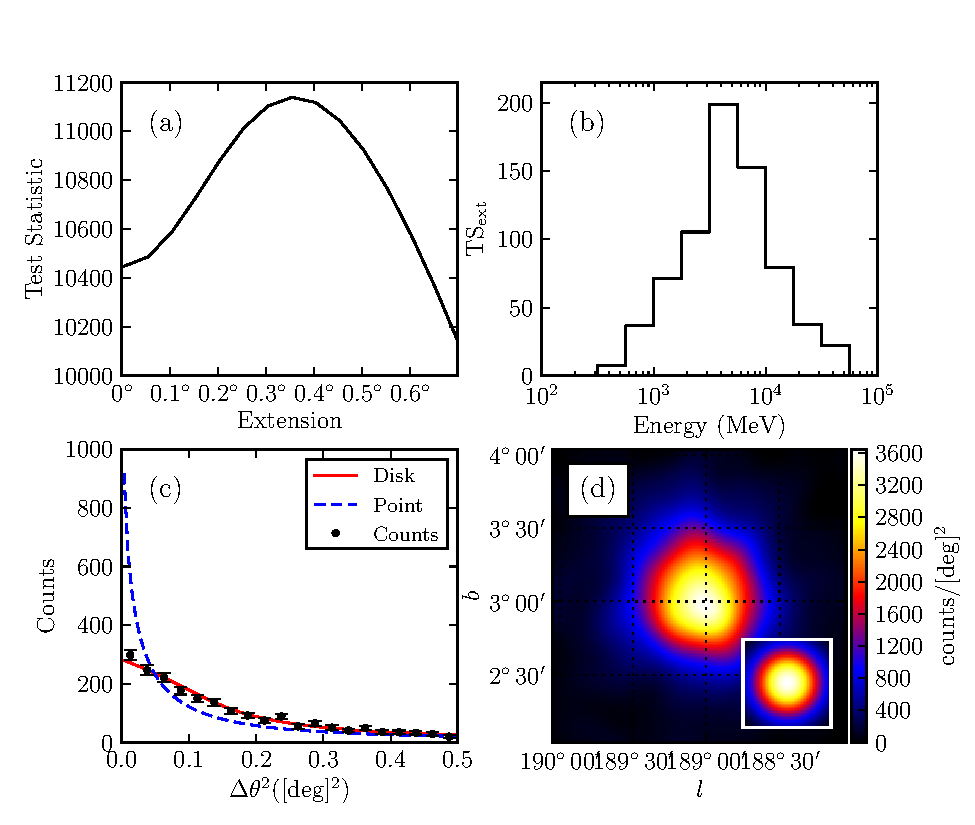
\includegraphics{ic443_plots/four_plots_ic443.pdf}
    % taken from /u/gl/lande/work/fermi/extended_catalog/2FGL/plots_for_paper/four_plots_ic443/v1/run.py
    \caption{
    All plots are for the SNR IC443 using two years of data.
    % ts vs extension
    Plot (a) is the change in \ts when varying the
    extension of the source.  
    % ts_ext vs energy
    Plot (b) is \tsext in twelve energy bins. This plot shows that there is
    little gain in sensitivity to the extension using photons
    with energies below 1 \gev, even for a source with an index $\approx2.4$.
    % radial integral
    Plot (c) is the sum of all counts within a given radial distance
    from the source binned uniformly in $\theta^2$. 
    Overlaid on the plot is the model predicted counts assuming that
    the source is both an extended source and a point source
    % smoothed counts
    Plot (d) is a counts map of the source with the Galactic and
    isotropic diffuse emission subtracted and smoothed by a $0.1\deg$
    Gaussian kernel.  The inset is the predicted emission from a point
    source of the same spectrum and intensity.  The PSF is smoothed
    by the same kernel.  Plots (a), (c), and (d) use only photons with
    energies between 1 \gev and 100 \gev. Plots (c) and (d)
    use only photons which converted in the front
    part of the detector and have an improved angular resolution.
    }
    \label{four_plots_ic443}
  \end{center}
\end{figure}

\begin{figure}
  \begin{center}
    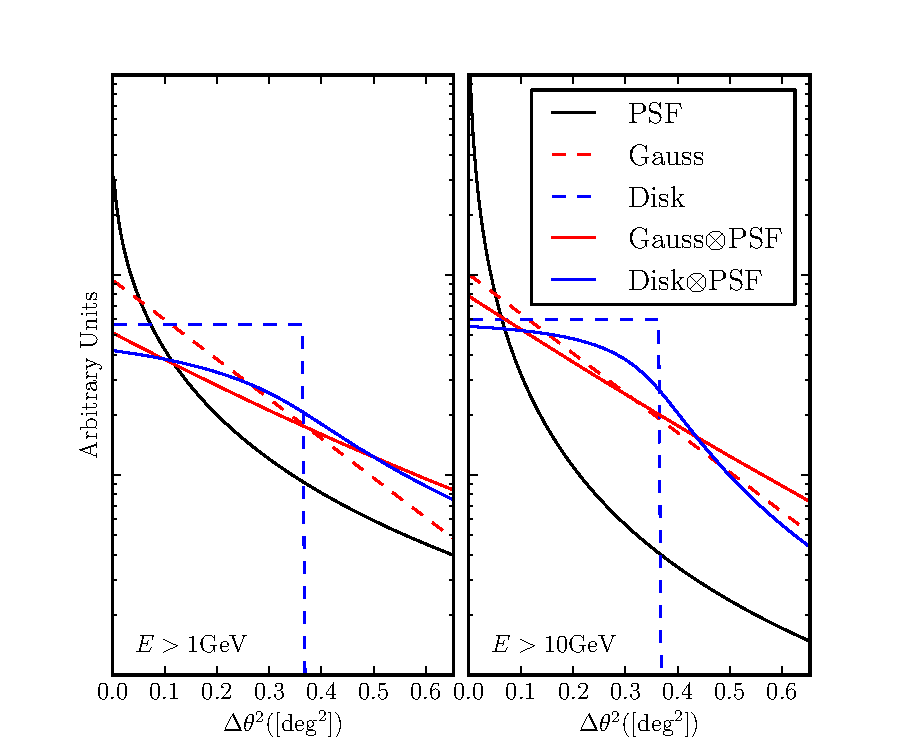
\includegraphics{mc_plots/compare_disk_gauss.pdf}
    % this plot came from /u/gl/lande/work/fermi/extended_catalog/2FGL/plots_for_paper/compare_disk_gauss/v2/compare_disk_gauss.pdf
    \end{center}
    \caption{
    A comparison of the Gaussian and uniform disk PDFs before and
    after convolving with the PSF.  The black line is the PSF that
    would be observed for a power-law source of spectral index 2. The
    dashed red line is the probability density of a Gaussian with
    $\rsixeight=0.5\deg$, which is just a straight line on this plot.
    The dashed blue line is the probability density for a uniform disk
    with $\rsixeight=0.5\deg$.  Finally, the solid red and blue lines
    show the convolution of the Gaussian and uniform disk with the PSF.
    Plot (a) shows the analysis in the energy range from 1 \gev to 100
    \gev while plot (b) shows the analysis only in the energy range
    from 10 \gev to 100 \gev. This plot demonstrates that different
    spatial models when smoothed by the PSF look similar.  The $y$
    axis is the log of the intensity and the $x$ axis is $\theta^2$.
    This plot is discussed further in section~\ref{compare_source_size}.
    }\label{compare_disk_gauss}
  \end{figure}

  \begin{figure}
    \begin{center}
      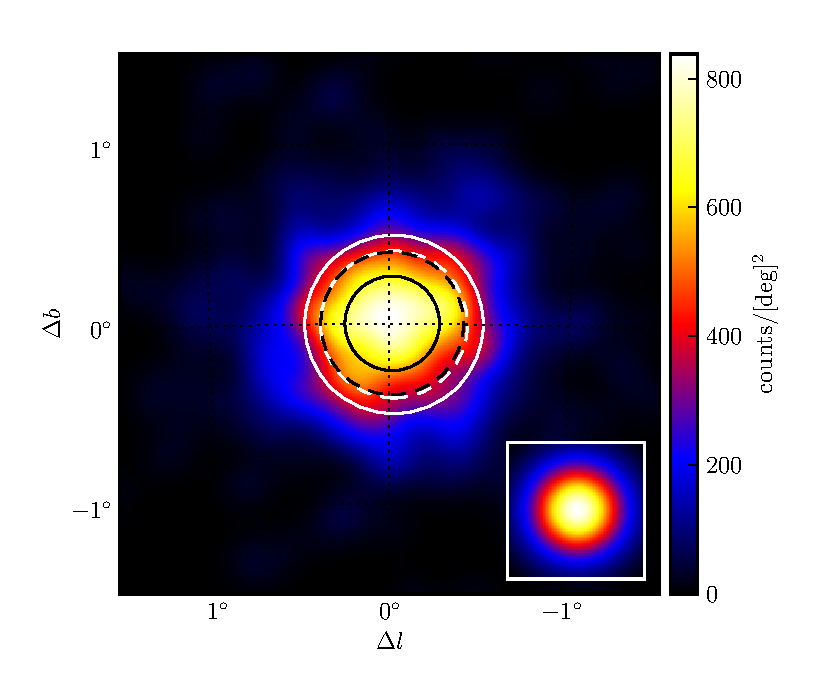
\includegraphics{mc_plots/compare_r68.pdf}
      % this plot came from /u/gl/lande/work/fermi/extended_catalog/2FGL/plots_for_paper/compare_r68/v2/plot.py
      \end{center}
      \caption{
      This plot shows that fitting the same source with different
      spatial shapes can lead to different values of the fitted
      extensions. On the other hand, the different shapes have a
      good agreement about the 68\% containment radius \rsixeight.
      It shows counts map for a simulated uniform disk extended source
      in the energy range from 1 \gev to 100 \gev.  The source has a
      size $\sigma=0.5\deg$, an integral flux between 1 \gev and 100
      \gev of $3\times 10^{-8}\ph/\cm^2/\sec$, and a spectral index 2.
      The smoothed counts from a point source with the same spectrum are
      shown in the bottom right inset.  This source was fit with both
      a uniform disk and a Gaussian spatial model.  The white circle
      represents the edge of the best fit uniform disk spatial model.
      The black circle is the fit $\sigma$ modeling the source with a
      Gaussian hypothesis.  The dashed white and black circle are the
      fit \rsixeight for the disk and Gaussian hypothesis. This plot is
      discussed further in section~\ref{compare_source_size}.
      }\label{compare_r68}
    \end{figure}


    \begin{table}
  \begin{centering}
    \begin{tabular}{ r | r | r | r }
      \hline
      \hline
      $\gamma$ & flux ($\ph/\cm^2/\sec$) & $N_\text{sims}$ & $\langle\ts\rangle$ \\
      \hline
      1.5 &          $10^{-6}$ &           31952 &  92862 \\
      &  $3\times 10^{-7}$ &           31962 &  22169 \\
      &          $10^{-7}$ &           31977 &   5806 \\
      &  $3\times 10^{-8}$ &           31991 &   1270 \\
      &          $10^{-8}$ &           31940 &    301 \\
      &  $3\times 10^{-9}$ &           30324 &     62 \\
      \hline
      2 &          $10^{-6}$ &           31872 &  22067 \\
      &  $3\times 10^{-7}$ &           31890 &   4898 \\
      &          $10^{-7}$ &           31858 &   1097 \\
      &  $3\times 10^{-8}$ &           31632 &    236 \\
      &          $10^{-8}$ &           27491 &    103 \\
      \hline
      2.5 &          $10^{-6}$ &           31822 &   4706 \\
      &  $3\times 10^{-7}$ &           31822 &    889 \\
      &          $10^{-7}$ &           31169 &    176 \\
      &  $3\times 10^{-8}$ &           21591 &     41 \\
      \hline                                                
      3 &          $10^{-6}$ &           31763 &    929 \\
      &  $3\times 10^{-7}$ &           31665 &    161 \\
      &          $10^{-7}$ &           19271 &     40 \\
      \hline
    \end{tabular}
    \caption{
    This table presents a list of the spectral models (flux and
    spectral index) used in the Monte Carlo study of \pointlike
    described in section~\ref{monte_carlo_validation} and presented
    in figure~\ref{ts_ext_mc}.  For each spectral model, the number of
    statistically independent simulations and the average value of \ts
    value ($\langle\ts\rangle$) is tabulated.  The Monte Carlo simulation
    spans parameters representative of sources that could be detected
    by the LAT.  The simulation is of spectral indices $\gamma$ of 1.5,
    2, 2.5, and 3.  The simulation is of fluxes varying from a $5\sigma$
    source detection to a $>10\sigma$ source detection.  Only simulations
    which produced statistically significant detections ($\ts>25$)
    were kept.  What is quoted is the $>100$ \mev integral flux measured
    in units of $\ph/\cm^2/\sec$.  More information about this Monte
    Carlo analysis is presented in section~\ref{monte_carlo_validation}.
    }\label{ts_ext_num_sims}
  \end{centering}
\end{table}

\clearpage

\clearpage
\begin{figure}
  \begin{center}
    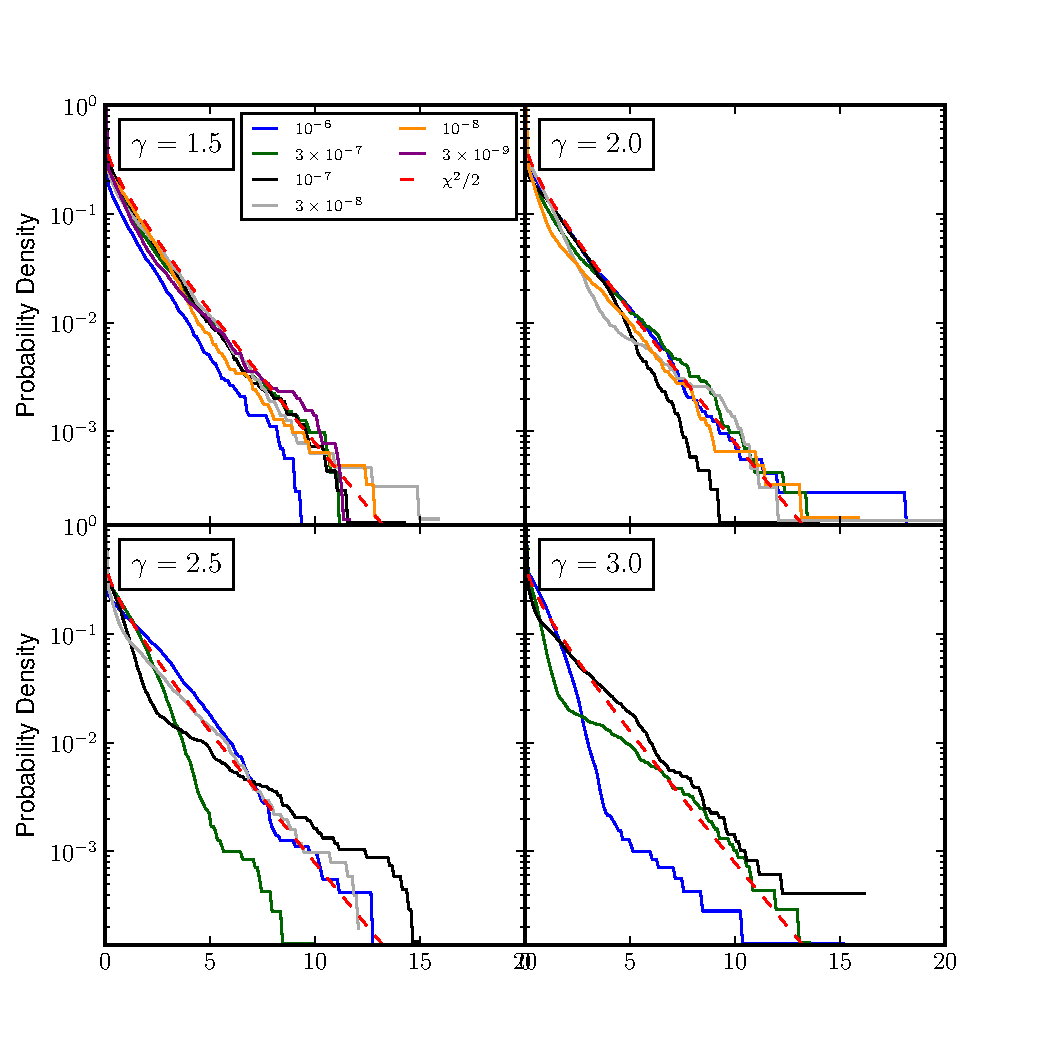
\includegraphics{mc_plots/ts_ext_emin_1000.pdf}
    % this plot came from /u/gl/lande/work/fermi/extended_catalog/monte_carlo/ts_ext/v3/plot.py
    % using data from /nfs/slac/g/ki/ki03/lande/extended_catalog/monte_carlo/ts_ext/v3_emin_1000/merged.hdf5
    \end{center}
    \caption{
     The plot shows the null distribution of
    the likelihood ratio test when fitting a point source for extension.
    The $x$ axis is \tsext and the $y$ axis is the cumulative density
    for \tsext of simulated point sources. The four plots represent
    different spectral indices and the different colors represent
    different fluxes.  The dashed red line is the cumulative density
    function of $\chi^2(\ts)/2$ which is suggested by Wilks' theorem
    as the distribution these curves should should follow.  There is
    good agreement between the Monte Carlo results and
    the theoretical distribution. For most spectral parameters, the
    Monte Carlo curve lies to the left of the theoretical curve which
    would make the theoretical distribution more conservative.  In this
    paper, we use this theoretical curve to estimate the significance of
    the detection of a source's extension. This plot cuts off 
    three simulations with $\tsext>25$. They 
    had a flux $3\times10^{-8}\ph/\cm^2/\sec$, spectral index
    2.5, and \tsext of 26.1, 28.9, and 38.1.
    The Monte Carlo simulation is described in 
    section \ref{monte_carlo_validation} and 
    the number of simulation for each spectral model 
    are presented in table~\ref{ts_ext_num_sims}.
    }\label{ts_ext_mc}
  \end{figure}

\clearpage

\begin{figure}
  \begin{center}
    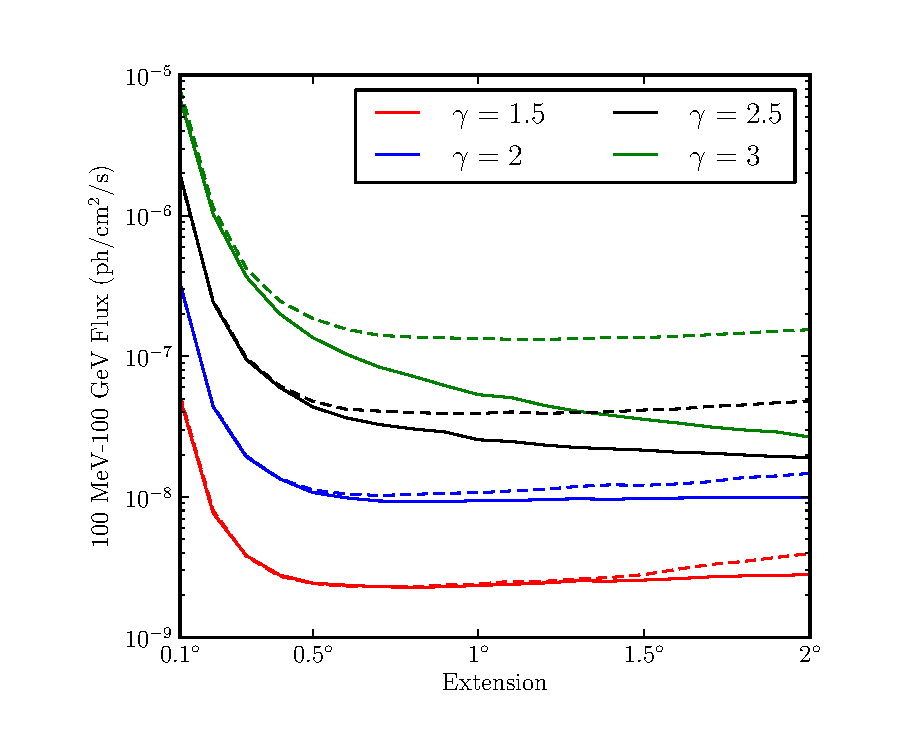
\includegraphics{mc_plots/index_sensitivity.pdf}
    % this plot came from /u/gl/lande/work/fermi/extended_catalog/monte_carlo/sensitivity/v12/plot/plot_vs_index.py
    \end{center}
    \caption{
    This plot shows the detection threshold to resolve a uniform
    disk extended source.  The detection threshold is defined as the flux where
    $\langle\tsext\rangle=16$ for a given extension.  The $x$ axis is
    the extension of a uniform disk extended source and the $y$ axis
    is the source's 100 \mev to 100 \gev photon flux.  All sources have
    an assumed power-law spectrum and the different colors are different
    simulated spectral indices.  The solid line is the detection threshold
    using photons with energy between 100 \mev and 100 \gev while the
    dashed line is the threshold using photons with energy between 1 \gev
    and 100 \gev.  The detection threshold is for the same two year time
    range as was used in 2FGL and in the following extended source search.
    The extended sources are simulated against
  a Sreekumar-like isotropic background.  More information
    about this plot is presented in section~\ref{extension_sensitivity}.
    This plot shows that our threshold to detecting the extension of
    a source is best for a source with size $~0.5\deg$. It also shows
    that for sources neither too large nor soft, our sensitivity is not
    significantly improved using photons with energy between 100 \mev
    and 1 \gev. More information about this plot is presented
    in section~\ref{extension_sensitivity}.
    }\label{index_sensitivity}
  \end{figure}

\clearpage

\begin{figure}
  \begin{center}
    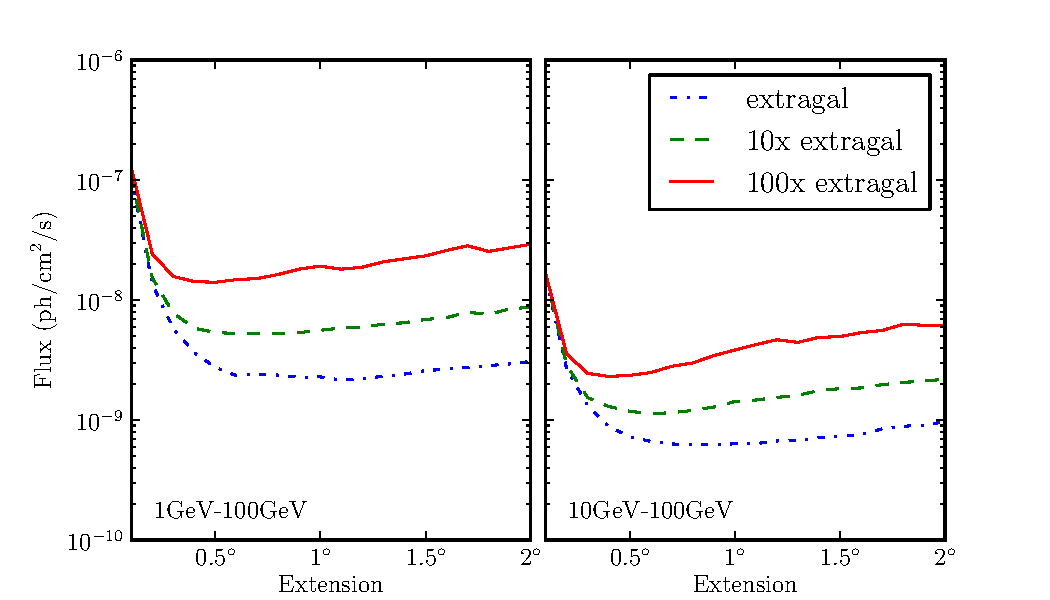
\includegraphics{mc_plots/diff_factor_sensitivity.pdf}
    % this plot came from /u/gl/lande/work/fermi/extended_catalog/monte_carlo/sensitivity/v12/plot/plot_vs_diff_factor.py
    \end{center}
    \caption{
    This shows the detection threshold to a uniform disk extended
    source for varying background levels
    and energy ranges.  The plots have the same meaning as in
    figure~\ref{index_sensitivity} and the simulations occur over the
    same time range.  The solid blue line is the detection threshold against a
    Sreekumar-like isotropic background. The green dashed curve is the
    threshold against 10 times the isotropic background and the dash
    dotted red curve is the threshold against 100 times the isotropic
    background.  The latter factor approximately represents the intensity
    of the Galactic diffuse emission near the Galactic center.  Plot (a)
    is the threshold using photons with energies between 1 \gev and 100
    \gev while plot (b) is the threshold using photons with energies
    between 10 \gev and 100 \gev. Unlike figure~\ref{index_sensitivity},
    the detection threshold was calculated only for a power-law source of spectral
    index 2. The flux is quoted only in the selected energy range which
    weakens the dependence of the detection threshold on spectral index.
    These plots show that we are less sensitive to extended sources in
    regions with higher background and (given the same number of photons)
    more sensitive to harder sources.  Overlaid on this plot are the
    extended sources found in this extended source search. The extended
    sources are color coded based upon whether the integral galactic
    diffuse and isotropic diffuse emission model is closer to 1x, 10x,
    or 100x the Sreekumar-like isotropic spectrum.  The red point
    in plot (a) below the red line is RX J1713.7-3946 which is harder
    ($\gamma\approx1.5$) and has diffuse emission only 53 times larger
    than the isotropic emission.  The green point in plot (b) below
    the green line is MSH 15-52 which was found by our analysis to
    have $\tsext=6.5$.  More information about this plot is presented
    in section~\ref{extension_sensitivity}.
    }\label{diff_factor_sensitivity}
  \end{figure}


\clearpage
\begin{figure}
  \begin{center}
    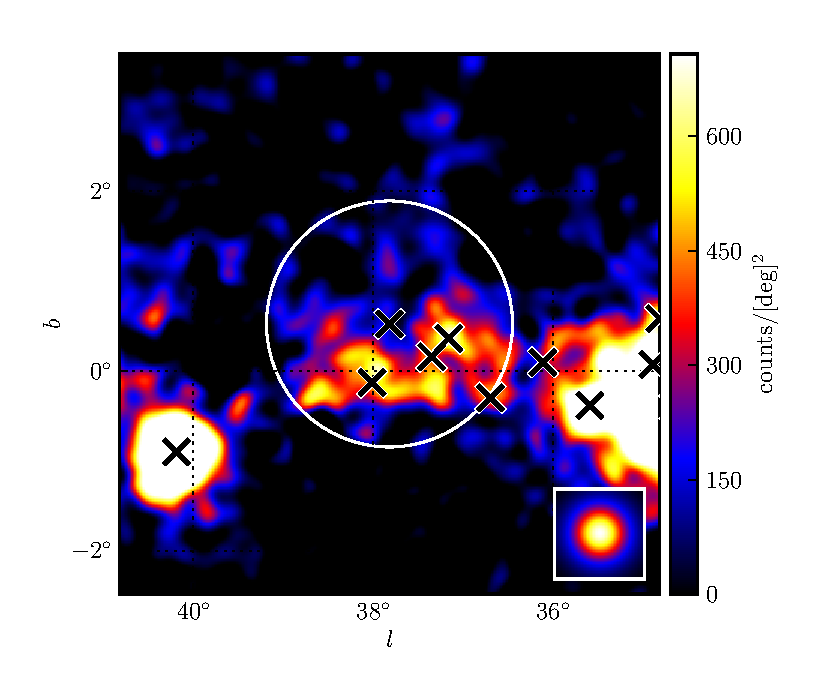
\includegraphics{source_plots/example_bad_fit.pdf}
    % taken from /u/gl/lande/work/fermi/extended_catalog/2FGL/plots_for_paper/example_bad_fit/v3/run.py
    \caption{
    The observed 1 \gev to 100 \gev photons for the two year catalog
    source 2FGL\,J1856.2+0450c. This map is smoothed by a 0.1\deg Gaussian
    kernel and the red cross and circle are the center and size of the
    best fit uniform disk spatial model. The result is statistically
    significant, but the extension encompasses many catalog sources and
    the emission does not look to be uniform. Instead, this source is
    probably fitting large-scale diffuse residual features. Although the
    fit is statistically significant, it is not physical and we manually
    discard candidates that appear like this.
    }
    \label{example_bad_fit}
  \end{center}
\end{figure}

\begin{figure}
  \begin{center}
  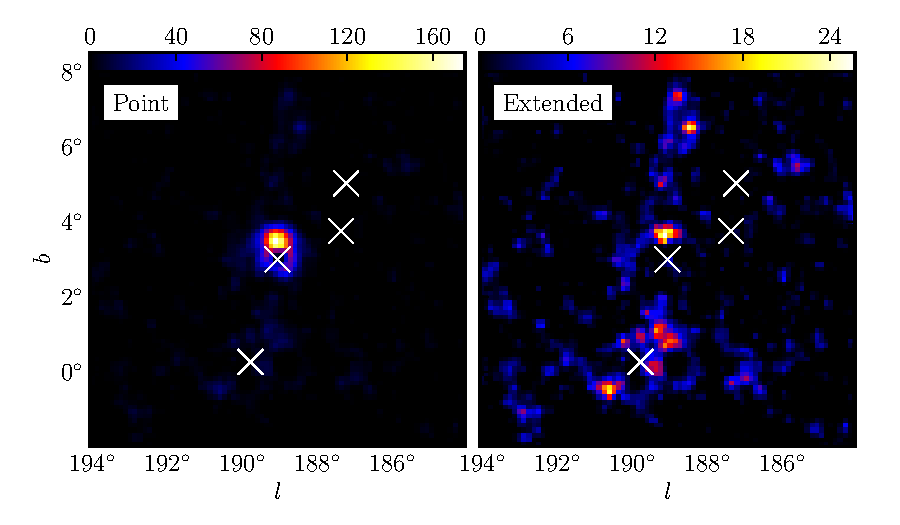
\includegraphics{ic443_plots/res_tsmap_ic443.pdf}
  % plot from /u/gl/lande/work/fermi/extended_catalog/2FGL/plots_for_paper/res_tsmap_ic443/v1

  \caption{An example residual test statistic map generated for the
  supernova remnant IC443 using photons with energy between 1 \gev
  and 100 \gev. Plot (a) is the residual \ts fitting IC443 as a point
  source and plot (b) is the residual TS fitting IC443 as an extended
  source. The crosses in the plot represent all of the sources modeled
  in the region. Since there is residual TS greater than 160 fitting
  with the point hypothesis so it is not a good model of the source.
  On the other hand, the residual fitting IC443 as an extended source
  is much lower because IC443 is better fit by an extended source. These
  plots were generated for all extended source candidates to help validate
  the analysis.}
  \label{res_tsmaps}
  \end{center}
\end{figure}


\clearpage
\begin{sidewaystable}
    \begin{centering}
      \begin{tabular}{l|rrlrrrrrrr}
        \hline
        \hline
        Name                 &          \glon &          \glat &                \multicolumn{1}{r}{$\sigma$} &         TS &   $\tsext$ &    Pos Err &                  Flux &                 Index  \\
        \hline
        \multicolumn{9}{c}{$E > 1 \gev$} \\
        \hline
        SMC                  &     302.68\deg &     -44.81\deg & $  1.75\deg \pm   0.07\deg \pm   0.02\deg $ &       94.8 &       67.4 &   0.12\deg & $    3.3 \pm     0.4$ & $   2.41 \pm    0.17$  \\
        LMC                  &     279.10\deg &     -32.61\deg & $  1.74\deg \pm   0.05\deg \pm   0.13\deg $ &     1101.3 &      860.5 &   0.05\deg & $   15.5 \pm     0.6$ & $   2.48 \pm    0.06$  \\
        IC443                &     189.05\deg &       3.04\deg & $  0.36\deg \pm   0.01\deg \pm   0.04\deg $ &    10719.8 &      510.4 &   0.01\deg & $   64.8 \pm     1.2$ & $   2.23 \pm    0.02$  \\
        Vela X               &     263.34\deg &      -3.11\deg & $                                 0.88\deg$ &            &            &            &                       &                       \\
        Centarus A           &     309.52\deg &      19.42\deg & $                            \approx10\deg$ &            &            &            &                       &                       \\
        W28                  &       6.50\deg &      -0.27\deg & $  0.43\deg \pm   0.02\deg \pm   0.03\deg $ &     1324.8 &      177.4 &   0.01\deg & $   58.0 \pm     1.8$ & $   2.63 \pm    0.03$  \\
        W30                  &       8.61\deg &      -0.20\deg & $  0.36\deg \pm   0.02\deg \pm   0.02\deg $ &      465.4 &       73.3 &   0.02\deg & $   30.7 \pm     1.6$ & $   2.59 \pm    0.04$  \\
        W44                  &      34.69\deg &      -0.38\deg & $  0.36\deg \pm   0.01\deg \pm   0.02\deg $ &     1903.3 &      217.7 &   0.01\deg & $   73.6 \pm     1.8$ & $   2.68 \pm    0.02$  \\
        W51C                 &      49.13\deg &      -0.45\deg & $  0.28\deg \pm   0.02\deg \pm   0.05\deg $ &     1819.5 &      115.7 &   0.01\deg & $   39.3 \pm     1.3$ & $   2.35 \pm    0.03$  \\
        Cygnus Loop          &      74.22\deg &      -8.46\deg & $  1.72\deg \pm   0.05\deg \pm   0.07\deg $ &      356.5 &      356.5 &   0.06\deg & $   11.1 \pm     0.7$ & $   2.53 \pm    0.11$  \\
        \hline
        \multicolumn{9}{c}{$E > 10 \gev$} \\
        \hline
        MSH 15-52            &     320.38\deg &      -1.22\deg & $  0.20\deg \pm   0.04\deg \pm   0.03\deg $ &       76.2 &        6.5 &   0.03\deg & $    0.6 \pm     0.7$ & $   2.27 \pm    0.73$  \\
        HESS J1825-137       &      17.56\deg &      -0.46\deg & $  0.65\deg \pm   0.03\deg \pm   0.01\deg $ &       83.6 &       55.9 &   0.05\deg & $    1.8 \pm     0.2$ & $   1.74 \pm    0.19$  \\
        \hline
        \hline
      \end{tabular}
      \caption{The twelve extended sources included in 2FGL.  The top
      list are the extended sources analyzed using photons with energies
      between 1 \gev and 100 \gev.  The lower table are the sources
      analyzed using photons with energies between 10 \gev and 100 \gev.
      The quoted flux is in units of $10^{-9}\ph/\cm^2/\sec$ and is the
      flux in the fit energy range (either 1-100 \gev or 10-100 \gev).
      All sources were fit using a uniform disk spatial template. The
      localization and extension were found using \pointlike while the
      TS and spectral values were calculated using \gtlike.  \ts and
      \tsext was computed with \gtlike assuming the best fit uniform
      disk spatial model from \pointlike.  \glon and \glat are Galactic
      longitude and latitude of the best fit extended source respectively.
      $\sigma$ is the edge of the best fit uniform disk spatial model.
      The first error on $\sigma$ is statistical and the second error
      is systematic (see section~\ref{systematic_errors_on_extension}).
      Pos Err is the error on the localization of the source.  Statistical
      errors are at the $1\sigma$ level.  The Vela X and the Centarus A
      Lobes were not fit by our anaysis but are include for completeness
      (\cite{velax,cen_a_lat}). More information about these sources is
      in section~\ref{validate_known}.
      }
      \label{known_extended_sources}
    \end{centering}
\end{sidewaystable}

\clearpage
\begin{figure}
  \begin{center}
    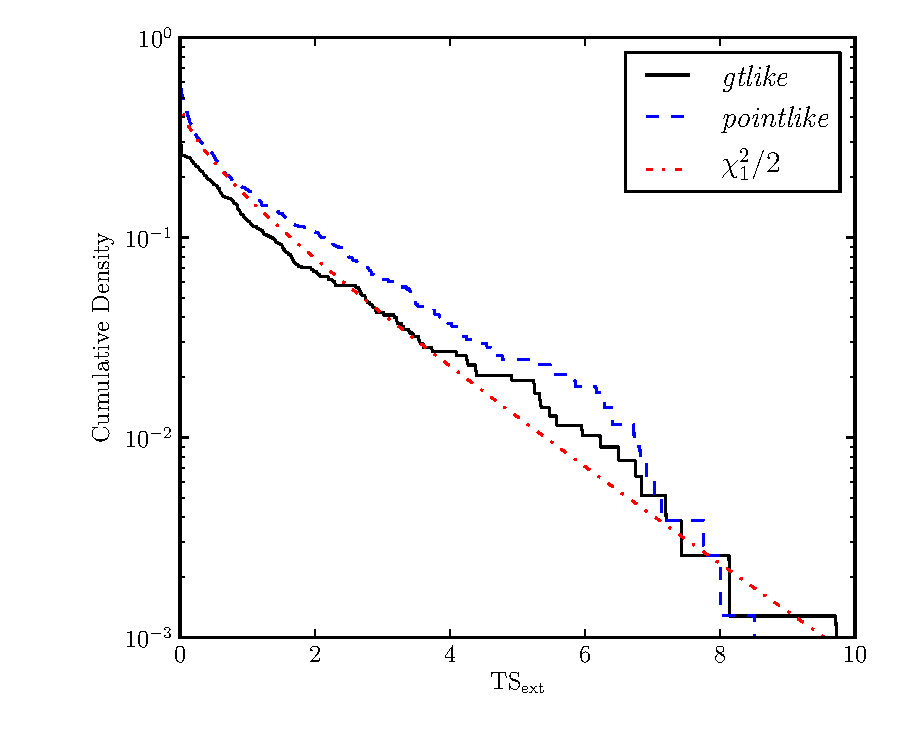
\includegraphics{source_plots/agn.pdf}
    % this plot came from /u/gl/lande/work/fermi/extended_catalog/2FGL/agn/v2/agn.py
    \end{center}
    \caption{The cumulative density of \tsext for 775 of
    the clean AGN in 2LAC which are significant above 1 \gev.
    AGN are expected to be unresolvable so overlaid on this plot
    is a $\chi^2/2$ distribution suggested by Wilks' theorem (see
    section~\ref{monte_carlo_validation}).  The \tsext distribution
    computed with \pointlike agrees with Wilks' theorem and confirms
    that we can use \tsext as a test of extension. The distribution
    computed by \gtlike is biased towards smaller values of \tsext. This
    is because \tsext is optimized using \pointlike and minor difference
    in the \pointlike and \gtlike likelihood function will cause the
    best fit model to be slightly different. Because \gtlike's curve
    lies to the left of the theoretical distribution, this makes our
    test conservative. More information about this analysis is presented
    in section~\ref{test_1lac_sources}.
    }\label{agn_ts_ext}
  \end{figure}


  % 1FGL J1628.6-2419c - P72Y2516         - 2FGL J1627.0-2425c
  % 1FGL J0823.3-4248  - P72Y1212         - 2FGL J0823.0-4246
  % 1FGL J1614.7-5138c - P72Y2473         - 2FGL J1615.2-5138
  % 1FGL J1632.9-4802c - P72Y2540         - 2FGL J1632.4-4753c
  % 1FGL J2020.0+4049  - P72Y3281         - 2FGL J2021.5+4026
  % 1FGL J1837.5-0659c - P72Y2974         - 2FGL J1837.3-0700c
  % N/A                - P72Y1287         - 2FGL J0851.7-4635


\clearpage
\thispagestyle{empty}
\begin{sidewaystable}
  \begin{centering}
    \begin{tabular}{l|rrlrrrrrrr}
      \hline
      \hline
      Name                 &          \glon &          \glat &                \multicolumn{1}{r}{$\sigma$} &         TS &   $\tsext$ &    Pos Err &                  Flux &                 Index &          Counterpart \\
      \hline
      \multicolumn{10}{c}{$E > 1 \gev$} \\
      \hline
      2FGL\,J0823.0-4246   &     260.32\deg &      -3.28\deg & $  0.37\deg \pm   0.03\deg \pm   0.02\deg $ &      320.9 &       46.3 &   0.02\deg & $    8.5 \pm     0.7$ & $   2.20 \pm    0.09$ &             Puppis A \\
      2FGL\,J1627.0-2425c  &     353.08\deg &      16.78\deg & $  0.41\deg \pm   0.05\deg \pm   0.02\deg $ &      144.5 &       31.1 &   0.04\deg & $    6.5 \pm     0.6$ & $   2.49 \pm    0.14$ &            Ophiuchus \\
      2FGL\,J1712.4-3941   &     347.25\deg &      -0.54\deg & $  0.56\deg \pm   0.04\deg \pm   0.01\deg $ &       75.0 &       39.6 &   0.05\deg & $    4.2 \pm     0.9$ & $   1.47 \pm    0.12$ &     RX\,J1713.7-3946 \\
      \hline
      \multicolumn{10}{c}{$E > 10 \gev$} \\
      \hline
      2FGL\,J0851.7-4635   &     266.29\deg &      -1.43\deg & $  1.13\deg \pm   0.08\deg \pm   0.05\deg $ &      116.1 &       87.2 &   0.07\deg & $    1.3 \pm     0.2$ & $   1.76 \pm    0.21$ &             Vela Jr. \\
      2FGL\,J1615.0-5051   &     332.38\deg &      -0.14\deg & $  0.33\deg \pm   0.04\deg \pm   0.01\deg $ &       53.4 &       16.3 &   0.04\deg & $    1.1 \pm     0.2$ & $   2.24 \pm    0.28$ &      HESS\,J1616-508 \\
      2FGL\,J1615.2-5138   &     331.66\deg &      -0.66\deg & $  0.42\deg \pm   0.03\deg \pm   0.01\deg $ &       76.6 &       48.0 &   0.05\deg & $    1.2 \pm     0.2$ & $   1.77 \pm    0.24$ &      HESS\,J1614-518 \\
      2FGL\,J1632.4-4753c  &     336.41\deg &       0.22\deg & $  0.44\deg \pm   0.04\deg \pm   0.03\deg $ &      127.8 &       64.5 &   0.04\deg & $    1.9 \pm     0.2$ & $   2.29 \pm    0.21$ &      HESS\,J1632-478 \\
      2FGL\,J1837.3-0700c  &      25.08\deg &       0.13\deg & $  0.35\deg \pm   0.08\deg \pm   0.03\deg $ &       46.2 &       18.8 &   0.07\deg & $    1.0 \pm     0.2$ & $   1.63 \pm    0.29$ &      HESS\,J1837-069 \\
      2FGL\,J2021.5+4026   &      78.18\deg &       2.19\deg & $  0.59\deg \pm   0.03\deg \pm   0.02\deg $ &      222.2 &      116.4 &   0.04\deg & $    1.8 \pm     0.2$ & $   2.31 \pm    0.19$ &          Gamma Cygni \\
      \hline
  \end{tabular}
    \caption{The 8 new source candidates found by the extended source
    search. Three new extended sources were found using photons with
    energies above 1 \gev and five new candidates were found using
    photons with energies above 10 \gev.  The columns in this table
    have the same meaning as in table~\ref{known_extended_sources}.
    More information about these sources can be found in
    section~\ref{new_ext_srcs_section}.
    }
    \label{new_ext_srcs_table}
  \end{centering}
\end{sidewaystable}



\clearpage
\begin{sidewaystable}
    \begin{centering}
      \begin{tabular}{l|rr|rrrr|rrrr}
        \hline
        \hline
        Name                 &     \tsinc &     \tsext &      $\glon_1$ &      $\glat_1$ &   $\text{Flux}_1$ &   $\text{Index}_1$ &      $\glon_2$ &      $\glat_2$ &   $\text{Flux}_2$ &  $\text{Index}_2$ \\
        \hline
        \multicolumn{11}{c}{$E > 1 \gev$} \\
        \hline
        2FGL\,J0823.0-4246   &       22.1 &       46.3 &     260.59\deg &      -3.27\deg & $       2.1 \pm        0.6$ & $  2.0 \pm   0.2$  &     260.24\deg &      -3.20\deg & $       5.4 \pm        0.7$ & $  2.4 \pm   0.2$ \\
        2FGL\,J1627.0-2425c  &       20.0 &       31.1 &     353.01\deg &      16.98\deg & $       3.1 \pm        0.6$ & $  2.6 \pm   0.3$  &     353.24\deg &      16.66\deg & $       2.5 \pm        0.6$ & $  2.5 \pm   0.4$ \\
        2FGL\,J1712.4-3941   &        6.4 &       39.6 &     347.28\deg &      -0.07\deg & $       0.2 \pm        0.1$ & $  0.6 \pm   0.5$  &     347.22\deg &      -0.27\deg & $       2.4 \pm        0.7$ & $  1.9 \pm   0.2$ \\
        \hline
        \multicolumn{11}{c}{$E > 10 \gev$} \\
        \hline
        2FGL\,J0851.7-4635   &       16.1 &       87.2 &     266.79\deg &      -1.32\deg & $       0.2 \pm        0.1$ & $  1.8 \pm   0.5$  &     266.41\deg &      -1.39\deg & $       0.2 \pm        0.1$ & $  1.5 \pm   0.6$ \\
        2FGL\,J1615.0-5051   &       11.9 &       16.3 &     332.39\deg &      -0.08\deg & $       0.4 \pm        0.1$ & $  2.3 \pm   0.6$  &     332.43\deg &      -0.36\deg & $       0.4 \pm        0.1$ & $  2.3 \pm   0.5$ \\
        2FGL\,J1615.2-5138   &       37.0 &       48.0 &     331.76\deg &      -0.37\deg & $       0.4 \pm        0.1$ & $  1.3 \pm   0.5$  &     331.47\deg &      -0.80\deg & $       0.4 \pm        0.1$ & $  2.0 \pm   0.4$ \\
        2FGL\,J1632.4-4753c  &       40.6 &       64.5 &     336.52\deg &       0.17\deg & $       0.7 \pm        0.2$ & $  2.8 \pm   0.5$  &     336.13\deg &       0.37\deg & $       0.5 \pm        0.1$ & $  1.7 \pm   0.4$ \\
        2FGL\,J1837.3-0700c  &       12.6 &       18.8 &      25.04\deg &       0.26\deg & $       0.3 \pm        0.1$ & $  1.2 \pm   0.5$  &      25.10\deg &      -0.05\deg & $       0.4 \pm        0.1$ & $  2.0 \pm   0.5$ \\
        2FGL\,J2021.5+4026   &       24.3 &      116.4 &      78.28\deg &       1.95\deg & $       0.3 \pm        0.1$ & $  5.0 \pm   0.0$  &      78.15\deg &       2.20\deg & $       0.6 \pm        0.1$ & $  1.7 \pm   0.4$ \\
        \hline
      \end{tabular}
      \label{dual_localization_results}
      \caption{For the new extended source candidates
      in table~\ref{new_ext_srcs_table}, we describe the
      results of the dual localization procedure described in
      section~\ref{dual_localization_method}. Here, the extended
      source candidate is not fit as an extended source but instead
      fit as two point sources.  The dual localization is performed
      with \pointlike and results in the best fit position of the two
      sources $(\glon_1,\glat_1)$ and $(\glon_2,\glat_2)$.  The change
      in likelihood and spectral values are then computed using \gtlike
      with the best fit positions found by \pointlike.  \tsinc is the
      increase in TS fitting the region as two sources compared to
      fitting compared to fitting a single point source and is computed
      using \gtlike with the best fit positions taken from \pointlike.
      It can be directly compared to \tsext, which is taken from
      table~\ref{new_ext_srcs_table}.  For all of our candidates, $\tsext
      > \tsinc$ which shows that an extended source fits the source better
      than two point sources.  As in table~\ref{known_extended_sources},
      flux is measured in units of $10^{-9}\ph/\cm^2/\sec$ and is the
      integral flux between 1 \gev (10 \gev) and 100 \gev for the sources
      found using photons above 1 \gev (10 \gev).}
    \end{centering}
  \end{sidewaystable}


  \clearpage
  \begin{sidewaystable}
    \begin{centering}
      \begin{tabular}{l|rrr|rrr|rrr}
        \hline
        \hline
        Name                 &     $\ts_\pointlike$ &        $\ts_\gtlike$ &       $\ts_\altdiff$ &      $\tsext_\pointlike$ &       $\tsext_\gtlike$ &    $\tsext_\altdiff$ &                $\sigma$ &       $\sigma_\altdiff$ &        $\sigma_\altpsf$ \\
        \hline
        \multicolumn{10}{c}{$E > 1 \gev$} \\
        \hline
        2FGL\,J0823.0-4246   &                350.9 &                320.9 &                352.5 &                     66.0 &                   46.3 &                 53.6 & $             0.37\deg$ & $             0.39\deg$ & $             0.38\deg$ \\
        2FGL\,J1627.0-2425c  &                170.2 &                144.5 &                112.6 &                     43.9 &                   31.1 &                 23.9 & $             0.41\deg$ & $             0.40\deg$ & $             0.39\deg$ \\
        2FGL\,J1712.4-3941   &                 80.9 &                 75.0 &                 43.4 &                     47.4 &                   39.6 &                 22.2 & $             0.56\deg$ & $             0.56\deg$ & $             0.54\deg$ \\
        \hline
        \multicolumn{10}{c}{$E > 10 \gev$} \\
        \hline
        2FGL\,J0851.7-4635   &                116.7 &                116.1 &                122.3 &                     87.1 &                   87.2 &                 90.4 & $             1.13\deg$ & $             1.16\deg$ & $             1.17\deg$ \\
        2FGL\,J1615.0-5051   &                 52.4 &                 53.4 &                 55.6 &                     17.5 &                   16.3 &                 17.4 & $             0.33\deg$ & $             0.32\deg$ & $             0.32\deg$ \\
        2FGL\,J1615.2-5138   &                 76.3 &                 76.6 &                 86.3 &                     44.0 &                   48.0 &                 52.6 & $             0.42\deg$ & $             0.43\deg$ & $             0.43\deg$ \\
        2FGL\,J1632.4-4753c  &                126.6 &                127.8 &                120.7 &                     63.9 &                   64.5 &                 64.1 & $             0.44\deg$ & $             0.44\deg$ & $             0.47\deg$ \\
        2FGL\,J1837.3-0700c  &                 45.4 &                 46.2 &                 39.0 &                     18.5 &                   18.8 &                 16.6 & $             0.35\deg$ & $             0.34\deg$ & $             0.38\deg$ \\
        2FGL\,J2021.5+4026   &                234.3 &                222.2 &                235.6 &                    135.9 &                  116.4 &                121.4 & $             0.59\deg$ & $             0.60\deg$ & $             0.60\deg$ \\
      \end{tabular}
      \caption{
      For the new extended sources, this table shows the results of
      fitting the new extended sources with an alternate diffuse model and
      an alternate PSF (see section~\ref{systematic_errors_on_extension}).
      It also compares the best fit results of \pointlike to \gtlike.
      $\ts_\pointlike$ and $\ts_\gtlike$, and $\ts_\altdiff$ are the \ts
      from \pointlike, \gtlike, and \gtlike with the alternate diffuse
      model respectively.  $\tsext_\pointlike$, $\tsext_\gtlike$, and
      $\tsext_\altdiff$ are the \tsext from \pointlike, \gtlike, and
      \gtlike with the alternate diffuse model respectively.  $\sigma$
      is the best fit extension using \pointlike and the standard PSF and
      diffuse model. $\sigma_\altdiff$ is the best fit extension using
      the alternate diffuse model and $\sigma_\altpsf$ is the best fit
      extension using the alternate PSF. The difference between
      these extensions is used to compute the systematic error
      on extension in table~\ref{known_extended_sources} and
      table~\ref{new_ext_srcs_table}.
      }\label{alt_diff_model_results}
    \end{centering}
  \end{sidewaystable}

\begin{figure}
  \begin{center}
    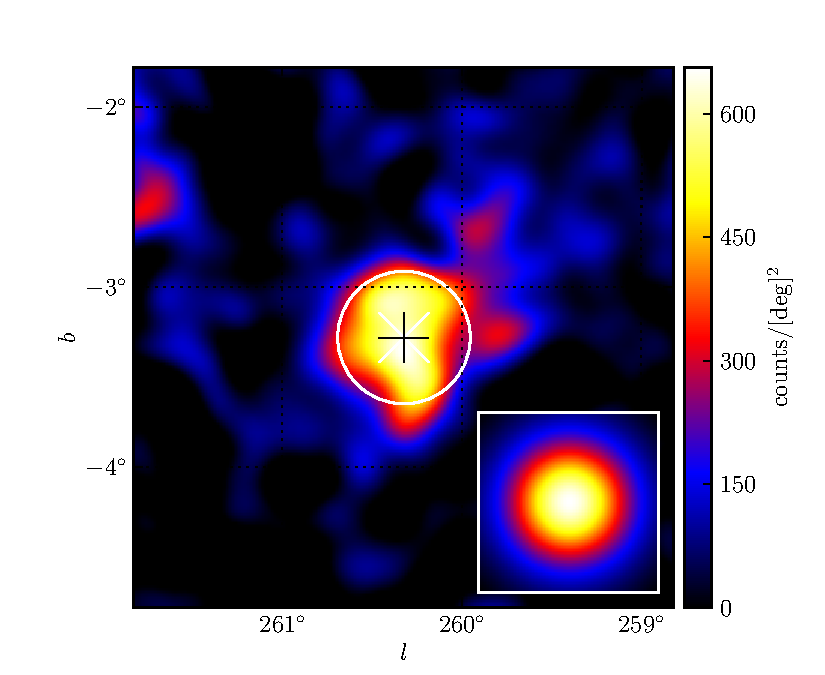
\includegraphics[type=pdf,ext=.pdf,read=.pdf]{source_plots/source_1FGL_J0823.3-4248}
  \end{center}
  % this plot came from 
  % /u/gl/lande/work/fermi/extended_catalog/2FGL/plots_for_paper/source_plots/1FGL_J0823.3-4248/v2/source_1FGL_J0823.3-4248.pdf
  \caption{A Galactic and isotropic diffuse subtracted 1-100
  \gev counts map of the region around 2FGL\,J0823.0-4246 smoothed by a
  0.1\deg Gaussian kernel.  The red star is the catalog position of this source.  
  The red cross and circle are the best fit position
  and extension of this source assuming a uniform disk spatial model.
  The two green stars are the positions of the sources 2FGL\,J0823.4-4305
  and 2FGL\,J0821.0-4254 which were removed because they are part of the
  extended source.  This source is spatially coincident with the Puppis
  A SNR. The light blue contours are an X-ray image of Puppis A observed by
  ROSAT (\cite{rosat_puppis_a}). There is good spatial overlap between
  the LAT and X-ray emission.  Even though the Vela pulsar is over 3
  degrees away from the source, because it is so bright it can be seen
  on the top left.  More information about this source can be found in 
  section~\ref{section_2FGL_J0823.0-4246}.
  }\label{1FGL_J0823.3-4248}
\end{figure}

\begin{figure}
  \begin{center}
    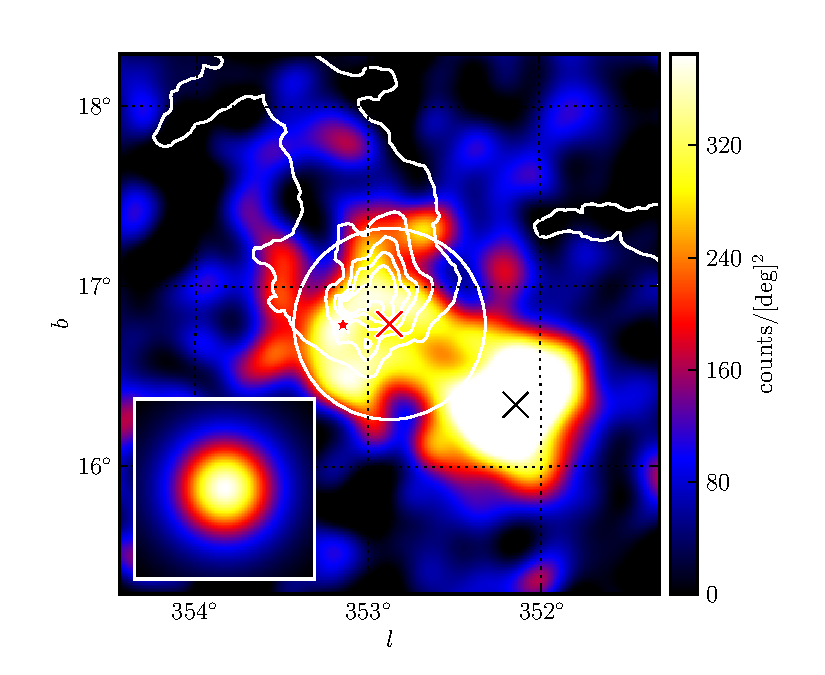
\includegraphics[type=pdf,ext=.pdf,read=.pdf]{source_plots/source_1FGL_J1628.6-2419c}
  \end{center}
  % this plot came from 
  % /u/gl/lande/work/fermi/extended_catalog/2FGL/plots_for_paper/source_plots/1FGL_J1628.6-2419c/v2/run.py
  \caption{
  A Galactic and isotropic diffuse subtracted 1-100 \gev counts
  map of the region around 2FGL\,J1627.0-2425 smoothed by a 0.1\deg
  Gaussian kernel.  Plot (a) has the diffuse emission model subtracted
  and plot (b) has the diffuse emission and 
  the background source 2FGL\,J1625.7-2526.  
  subtracted.  The red star is the catalog's position of this source.
  The red cross and circle are the best position and extension of
  this source assuming a uniform disk spatial model.  The light
  blue contours are from a 100 micrometer infrared image of the region
  as seen by IRAS (\cite{iras_rho_ophiuci}). This source is in the
  Ophiuchus region and most likely represents unmodeled diffuse
  emission.  More information about this source can be found in
  section~\ref{section_2FGL_J1627.0-2425c}.
  }\label{1FGL_J1628.6-2419c}
\end{figure}

\begin{figure}
  \begin{center}
    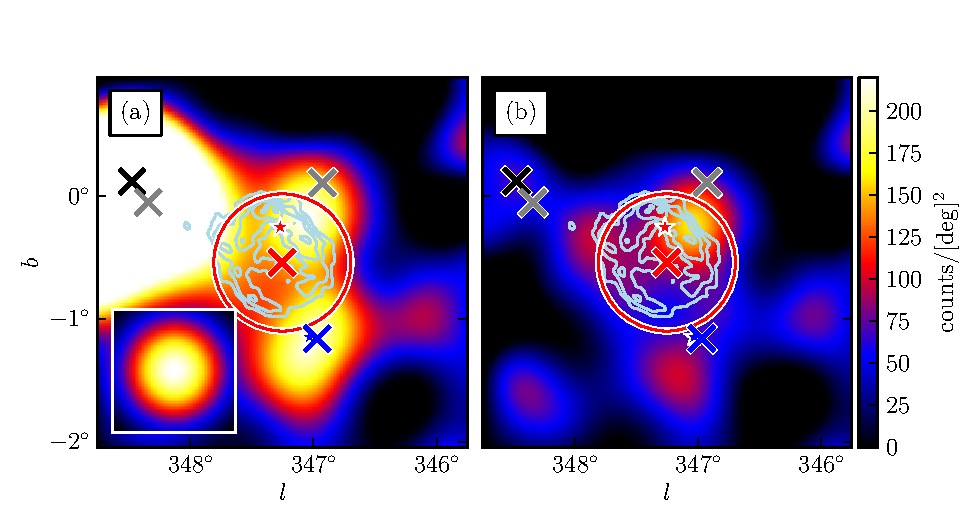
\includegraphics[type=pdf,ext=.pdf,read=.pdf]{source_plots/source_RX_J1713.7-3946}
    % this plot came from
  % /u/gl/lande/work/fermi/extended_catalog/2FGL/plots_for_paper/source_plots/RX_J1713.7-3946/v6/run.py
  \end{center}
  \caption{A Galactic and isotropic diffuse subtracted 1-100 \gev
  counts map of the region around 2FGL\,J1712.4-3941 smoothed by
  a 0.25\deg Gaussian kernel.  Plot (a) has the diffuse emission
  model subtracted and plot (b) has the diffuse emission and all
  background sources subtracted.  This source is spatially
  coincident with RX J1713.7-3946 was was recently reported by
  (\cite{rx_j1713_lat}).  The light blue contours are from the \tev image
  observed by H.E.S.S. (\cite{rx_j1713_hess}).  The region was analyzed
  with the same background model as (\cite{rx_j1713_lat}).  Source A (blue
  cross) is spatially coincident with 2FGL\,J1715.4-4024c (blue star).
  The grey crosses represent from left to right the position of source B
  and C which were added to the background model. More information about
  this source can be found in section~\ref{section_2FGL_J1712.4-3941}.
  }\label{2FGL_J1712.4-3941}
\end{figure}



\begin{figure}
  \begin{center}
    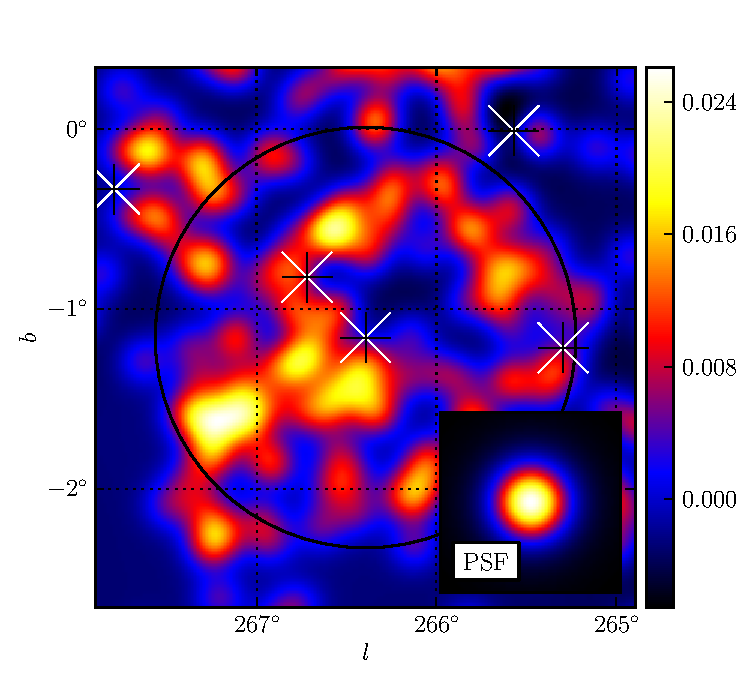
\includegraphics[type=pdf,ext=.pdf,read=.pdf]{source_plots/source_Vela_Jr}
  \end{center}
  % this plot came from 
  % /u/gl/lande/work/fermi/extended_catalog/2FGL/plots_for_paper/source_plots/Vela_Jr/v2/source_Vela_Jr.pdf
  \caption{A Galactic and isotropic diffuse subtracted 10-100
  \gev counts map of the region around 2FGL\,J0851.7-4635 smoothed
  by a 0.25\deg Gaussian kernel. This image is smoothed by a larger
  kernel because it is significantly larger than the other sources.
  The red star is the catalog position of this source.  The red cross
  and circle are the best fit position and extension of the source
  assuming a uniform disk spatial model.  The inner three green stars
  are (from left to right) 2FGL\,J0853.5-4711, 2FGL\,J0855.4-4625,
  and 2FGL\,J0848.5-4535 which were removed because they are part of
  the extended source.  The farther away green stars are (from left to
  right) 2FGL\,J0901.7-4655 and 2FGL\,J0858.0-4815 which were removed
  because they were not significant above 10 \gev.  The blue cross
  is the relocalized position of 2FGL\,J0854.7-4501.  This extended
  source is spatially coincident with the Vela Jr SNR.  The light
  blue contours are from the \tev image of Vela Jr. observed by H.E.S.S
  (\cite{vela_jr_hess}).  More information about this source can be
  found in section~\ref{section_2FGL_J0851.7-4635}.
  }\label{Vela_Jr}
\end{figure}

\begin{figure}
  \begin{center}
    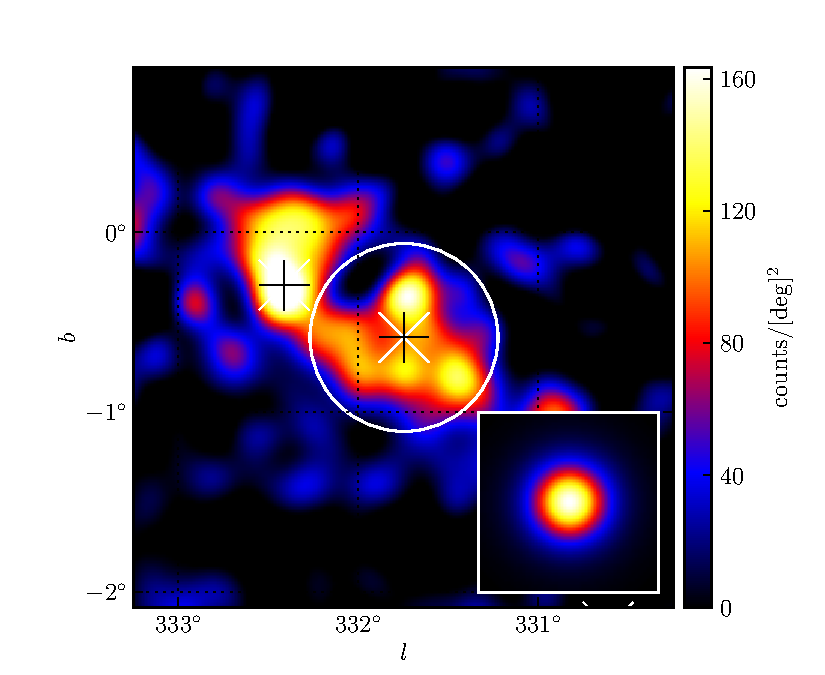
\includegraphics[type=pdf,ext=.pdf,read=.pdf]{source_plots/source_1FGL_J1613.6-5100c}
  \end{center}
  % this plot came from 
  % /u/gl/lande/work/fermi/extended_catalog/2FGL/plots_for_paper/source_plots/1FGL_J1613.6-5100c/v2/source_1FGL_J1613.6-5100c.pdf
  \caption{
    A Galactic and isotropic diffuse subtracted 10-100
    \gev counts map of the region around 2FGL\,J1615.0-5051 (upper
    left) and 2FGL\,J1615.2-5138 (lower right) smoothed by a 0.1\deg
    Gaussian kernel.  The red stars are the catalog positions of these
    sources.  The red stars and circles are the best fit positions and
    extensions of these sources assuming uniform disk spatial models.
    The green star inside the extension of 2FGL\,J1615.2-5138  is
    2FGL\,J1614.9-5212 which was removed because it is part of the
    extended source.  The green stars to the left are 2FGL\,J1619.7-5040c
    and 2FGL\,J1620.6-5111c which were removed because they were
    not significant above 10\gev. These are shown as green stars.
    The light blue
    contours are from the \tev image 
    of the extended sources
    HESS\,J1616-508 (left) and the extended source HESS\,J1614-518
    (right)
    observed by H.E.S.S
    (\cite{hess_plane_survey})
    2FGL\,J1615.0-5051 is spatially consistent with HESS\,J1616-508 and
    2FGL\,J1615.2-5138 is spatially consistent with HESS\,J1614-518.
    Figure~\ref{hess_seds} (a) and (b) shows the \gev and \tev SEDs for
    these sources.
    More information about 2FGL J1615.0-5051 can be found in
    section~\ref{section_2FGL_J1615.0-5051} and 2FGL\,J1615.2-5138 in
    section~\ref{section_2FGL_J1615.2-5138}.
  }\label{1FGL_J1613.6-5100c}
\end{figure}

\begin{figure}
  \begin{center}
    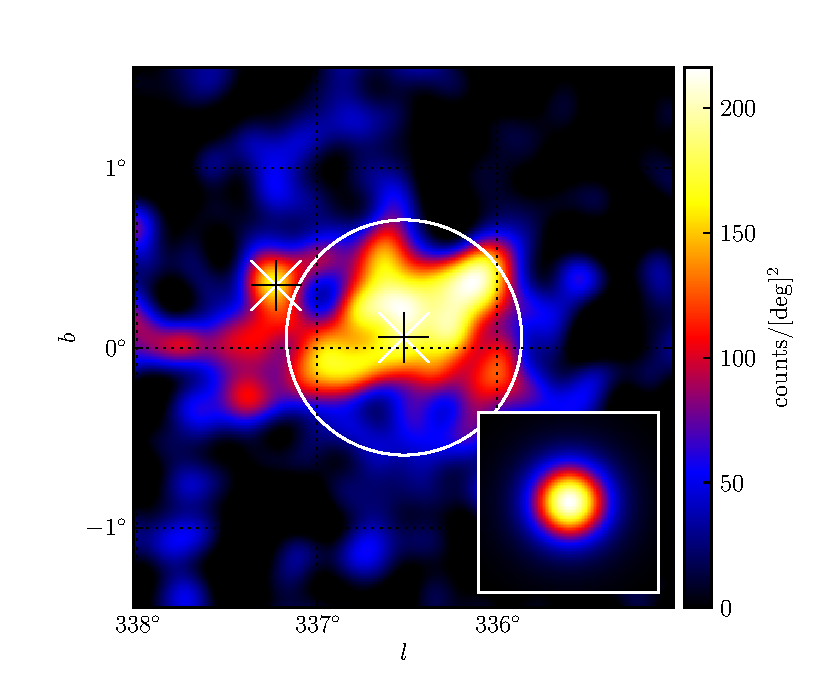
\includegraphics[type=pdf,ext=.pdf,read=.pdf]{source_plots/source_1FGL_J1632.9-4802c}
  \end{center}
  % this plot came from 
  % /u/gl/lande/work/fermi/extended_catalog/2FGL/plots_for_paper/source_plots/1FGL_J1632.9-4802c/v2/source_1FGL_J1632.9-4802c.pdf
  \caption{A Galactic and isotropic diffuse subtracted 10-100
  \gev counts map of the region around 2FGL\,J1632.4-4753c smoothed by
  a 0.1\deg Gaussian kernel.  This source is in a crowded region.
  The red star is the catalog position of this source.  The red
  cross and circle are the best fit position and extension 2FGL
  J1632.4-4753c assuming a uniform disk spatial model.  The three
  green crosses inside the extension are 2FGL
  J1631.7-4720c, 2FGL\,J1630.2-4752, and 2FGL\,J1634.4-4743c.4-4820c
  which were removed because they are part
  of the extended source.  The blue stars and crosses are the catalog
  positions and the relocalized positions of (from left to right)
  2FGL\,J1635.4-4717c and 2FGL\,J1636.3-4740c.  The farther away green
  stars are other catalog sources which were removed because they are
  not significant above 10 \gev.  This extended source is spatially
  coincident with the extended H.E.S.S source HESS\,J1632-478.
  The light blue contours are from the \tev image observed by H.E.S.S.
  (\cite{hess_plane_survey}).  Figure~\ref{hess_seds} (c) shows the \gev and
  \tev SED for this source.  More information about this source can be
  found in section~\ref{section_2FGL_J1632.4-4753c}.
  }\label{1FGL_J1632.9-4802c}
\end{figure}


\begin{figure}
  \begin{center}
    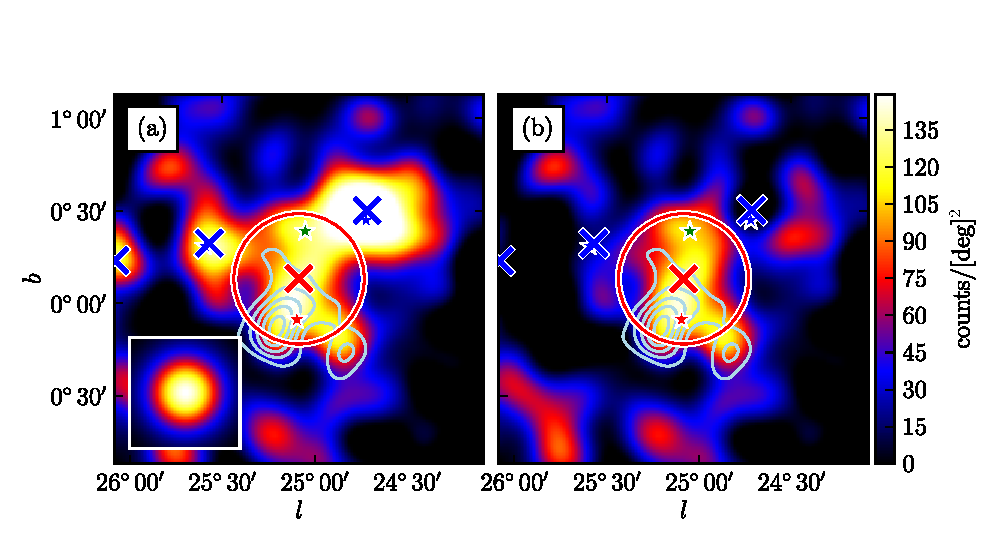
\includegraphics[type=pdf,ext=.pdf,read=.pdf]{source_plots/source_1FGL_J1837.5-0659c}
  \end{center}
  % this plot came from 
  % /u/gl/lande/work/fermi/extended_catalog/2FGL/plots_for_paper/source_plots/1FGL_J1837.5-0659c/v2/source_1FGL_J1837.5-0659c.pdf
  \caption{
  A Galactic and isotropic diffuse subtracted 10-100 \gev counts map of
  the region around 2FGL\,J1837.3-0700c smoothed by a 0.1\deg Gaussian
  kernel.  Plot (a) has the diffuse emission model subtracted and plot (b)
  has the diffuse emission and all background sources subtracted.  The red
  star is the catalog position of this source. The red cross and circle
  are the best fit position and extension  of 2FGL\,J1837.3-0700c assuming
  a uniform disk spatial model.  The blue stars and crosses are the
  catalog position and the relocalized position of (from left to right)
  2FGL\,J1839.3-0558c, 2FGL\,J1836.8-0623c, and 2FGL\,J1834.7-0705c.
  The green cross inside the extension is 2FGL\,J1835.5-0649 which
  was removed because it is part of the extended source.  The farther
  away green star is 2FGL J1839.0-0539 which was removed because
  it is not significant above 10 \gev.  This source is spatially
  coincident with the \tev source HESS\,J1837-069.  The light blue contours are from the \tev image observed by H.E.S.S.
  (\cite{hess_plane_survey}).  Figure~\ref{hess_seds} (d) shows the \gev
  and \tev SED for this source.  More information about this source can
  be found in section~\ref{section_2FGL_J1837.3-0700c}.
  }\label{1FGL_J1837.5-0659c}
\end{figure}


\begin{figure}
  \begin{center}
    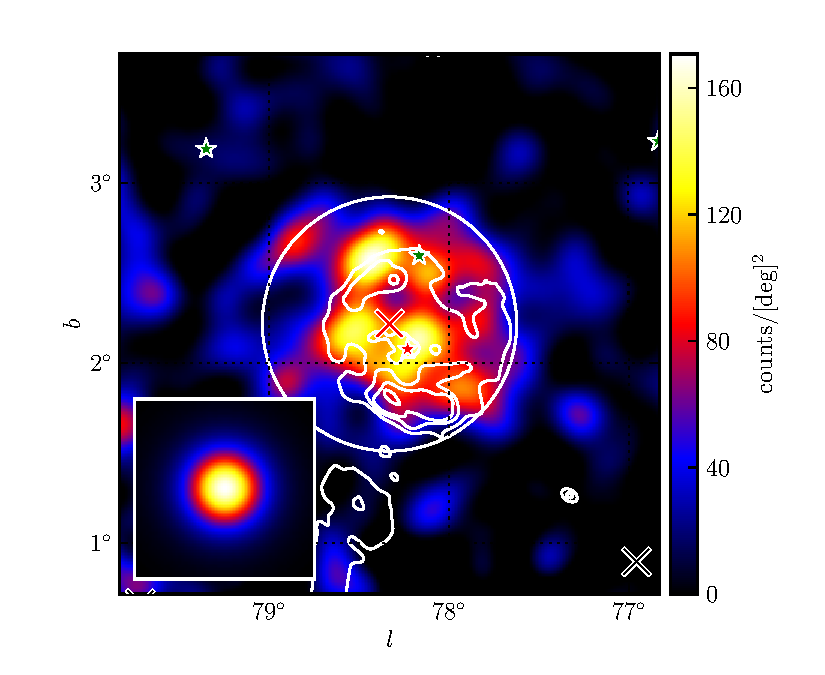
\includegraphics[type=pdf,ext=.pdf,read=.pdf]{source_plots/source_Gamma_Cygni}
  \end{center}
  % this plot came from 
  % /u/gl/lande/work/fermi/extended_catalog/2FGL/plots_for_paper/source_plots/Gamma_Cygni/v2/source_Gamma_Cygni.pdf
  \caption{A Galactic and isotropic diffuse subtracted 10-100
  \gev counts map of the region around 2FGL\,J2021.5+4026 smoothed by a
  0.1\deg Gaussian kernel. The red star is the catalog position of 2FGL
  J2021.5+4026.  The red cross and circle are the best fit position and
  extension 2FGL\,J2021.5+4026 assuming a uniform disk spatial model.
  The green cross inside the extension is 2FGL\,J2019.1+4040 which
  was removed because it is part of the extended source.  The farther
  away green stars represent other catalog sources which were removed
  because they were not significant above 10 \gev.  The grey cross is
  the position a source not in the two year catalog which was added
  to the region. 2FGL\,J2021.5+4026 is spatially coincident with the
  Gamma Cygni SNR.  The light blue contours are from a 408MHz image of Gamma Cygni
  observed by the Canadian Galactic Plane Survey.  More information about
  this source can be found in section~\ref{section_2FGL J2021.5+4026}.
  }\label{1FGL_J2020.0+4049}
\end{figure}

\clearpage
\begin{figure}
  \begin{center}
    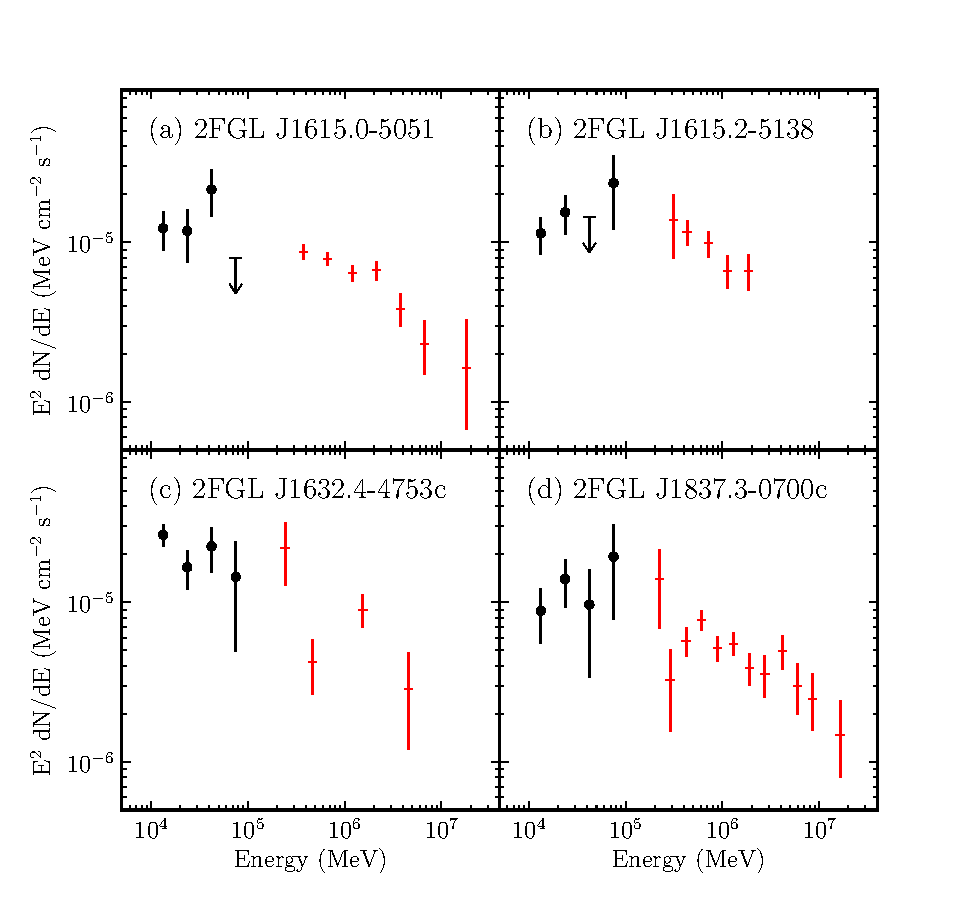
\includegraphics{summary_plots/hess_seds.pdf}
    % this plot came from /u/gl/lande/work/fermi/extended_catalog/2FGL/seds/v2/plot_seds/plot_seds.py
    \end{center}
    \caption{
    The spectral energy distribution of four the extended sources
    associated with extended \tev sources.  The black points with circular
    markers are the LAT data points. The red points with dashed markers
    are H.E.S.S points of associated sources.  Plot (a) shows the \gev
    SED of 2FGL\,J1615.0-5051 and the \tev SED of HESS\,J1616-508.
    Plot (b) shows 2FGL\,J1615.2-5138 and HESS\,J1614-518 Plot (c)
    shows 2FGL\,J1632.4-4753c and HESS\,J1632-478. Plot (d) shows
    2FGL\,J1837.3-0700c and HESS\,J1837-069. The H.E.S.S. data points
    are from (\cite{hess_plane_survey}) The LAT upper limits are at the
    95\% confidence level.  Both LAT and H.E.S.S. spectral errors are
    systematic only.
    }\label{hess_seds}
  \end{figure}

\clearpage
\begin{sidewaysfigure}
  \begin{center}
    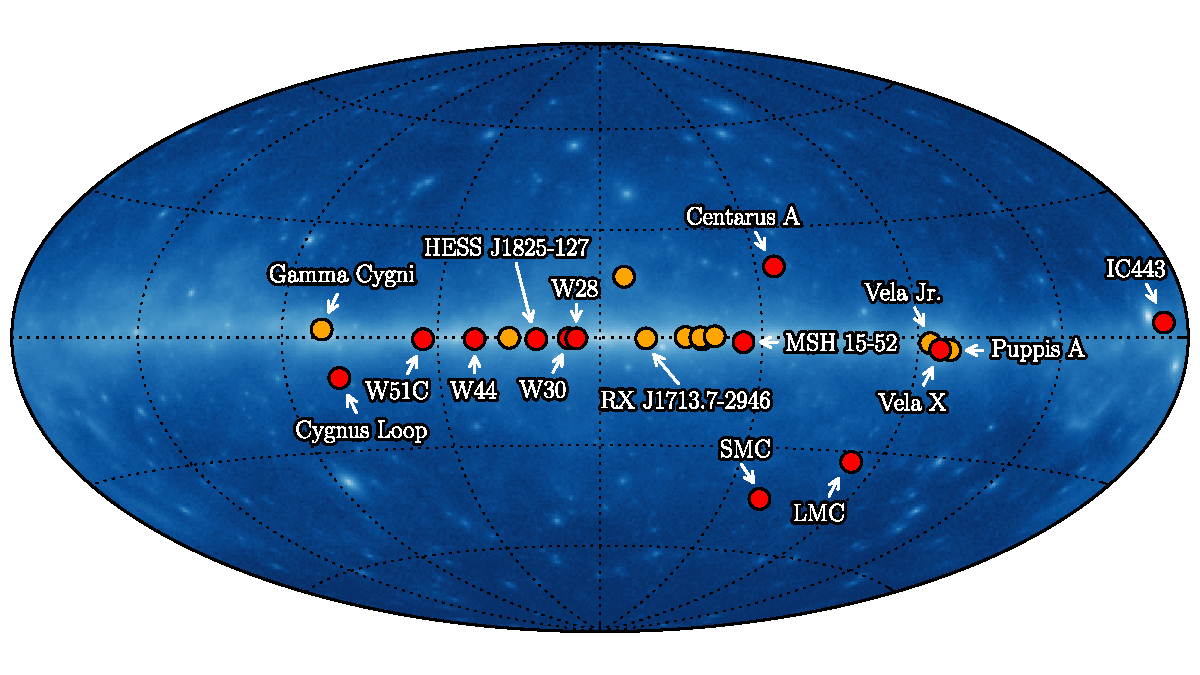
\includegraphics{summary_plots/allsky_extended_sources.pdf}
    % this plot came from /u/gl/lande/work/fermi/extended_catalog/2FGL/plots_for_paper/allsky/v1/run.py
    \end{center}
    \caption{A plot of all \gev extended sources detected by the LAT
    with two years of data.  The twelve extended sources included in
    2FGL are the red markers and the nine additional
    extended sources analyzed in this paper are the orange markers. The
    extended sources are overlaid on an Aitoff projection Galactic
    coordinate map of all 100 \mev to 100 \gev photons measured by the
    LAT in the two year time interval of this analysis.
    }\label{allsky_extended_sources}
  \end{sidewaysfigure}

\clearpage
\begin{figure}
  \begin{center}
    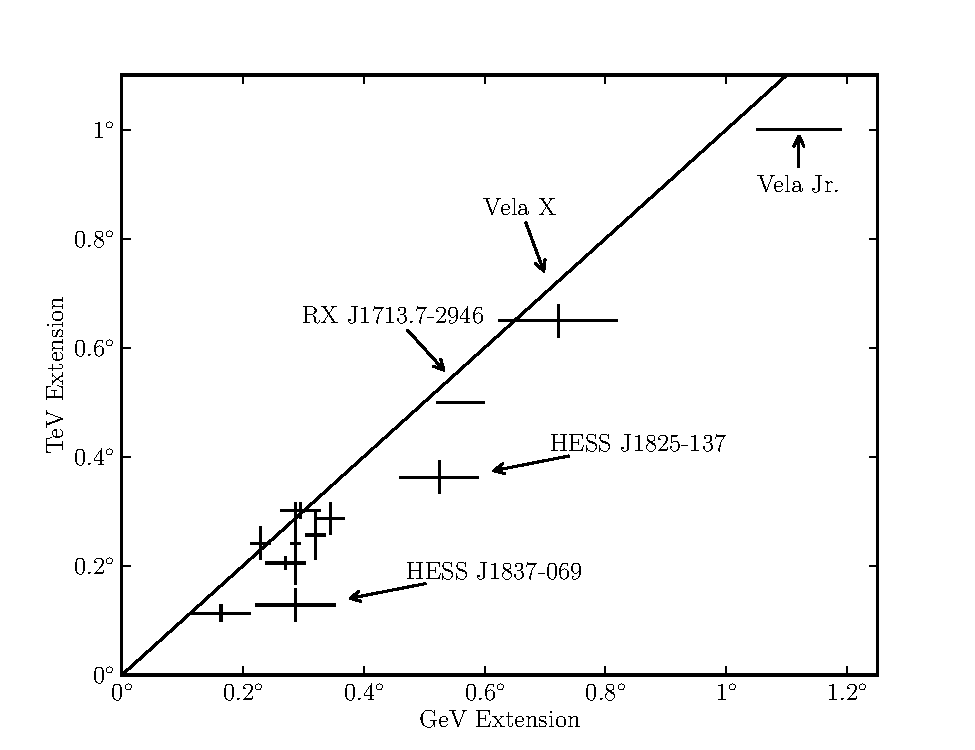
\includegraphics{summary_plots/gev_vs_tev_plot.pdf}
    % this plot came from /u/gl/lande/work/fermi/extended_catalog/2FGL/plots_for_paper/compare_tev_gev_sizes/v1/run.py
    \end{center}
    \caption{
    A comparison of the \gev and \tev sizes of LAT extended
    sources detected by \tev instruments.  The \tev extensions
    of W30, 2FGL\,J1837.3-0700c, 2FGL\,J1632.4-4753c,
    2FGL\,J1615.0-5051, and 2FGL\,J1615.2-5138 are from the
    H.E.S.S. Galactic plane survey (\cite{hess_plane_survey}).
    The \tev extensions of MSH 15-52, HESS\,J1825-137, Vela X,
    Vela Jr., RX J1713.7-3946 and W28 are respectively from H.E.S.S.
    (\cite{msh_15_52_hess,hess_j1825_hess,vela_x_hess,vela_jr_hess,rx_j1713_hess,w28_hess}).
    The \tev extension of IC443 is from Veritas (\cite{ic443_veritas})
    and W51c is from Magic (\cite{w51c_with_magic_at_fermi_symposium}).
    The LAT extension of Vela X is from (\cite{velax}).  Except for RX
    J1713.7-3946 Vela Jr., the \tev sources were fit with a Gaussian
    spatial model so the plotted \gev and \tev extensions were first
    converted to \rsixeight (see section~\ref{compare_source_size}).
    Because of their large size, the RX J1713.7-3946 and Vela Jr.
    were not directly fit in \tev. The \tev radius of RX J1713.7-3946
    is taken to be 0.5\deg and Vela Jr. to be 1\deg and the LAT size
    is not converted to \rsixeight. The LAT extension errors are
    the statistical and systematic errors added in quadrature. This
    plot shows that there is a correlation between the \gev and \tev
    sizes of sources.  The \tev size of MSH 15-52, HESS\,J1614-518,
    HESS\,J1632-478, and HESS\,J1837-069 have only been reported with
    an elliptical Gaussian fit and so the plotted size is the average
    of semi-major and semi-minor axis.
    }\label{gev_vs_tev_plot}
  \end{figure}

\clearpage
\begin{figure}
  \begin{center}
    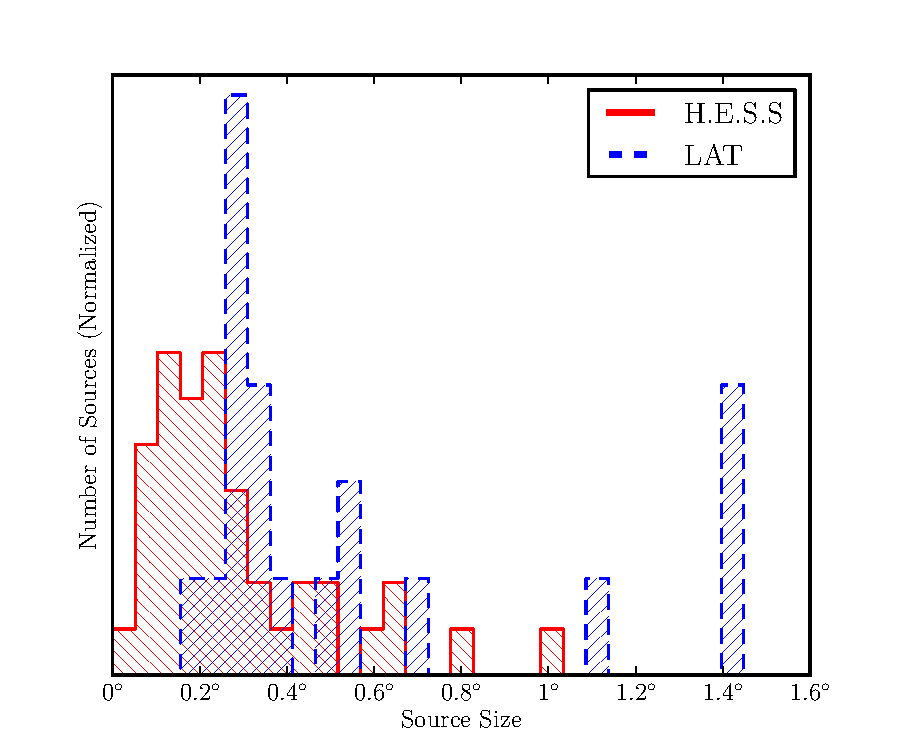
\includegraphics{summary_plots/gev_vs_tev_histogram.pdf}
    % this plot came from /u/gl/lande/work/fermi/extended_catalog/2FGL/plots_for_paper/extension_histogram/v4/extension_histogram.py
    \end{center}
    \caption{
    A comparison of the size of detected LAT and H.E.S.S sources.
    The extension of the 22 extended LAT sources comes from
    table~\ref{known_extended_sources}, table~\ref{new_ext_srcs_table},
    and the LAT extension of Vela X is taken from (\cite{velax}). The
    Centarus A lobes, which have an extension $~10\deg$, are not
    included in the plot (\cite{cen_a_lat}).  The \tev extension of
    the 42 extended H.E.S.S. sources comes from the H.E.S.S. Source
    Catalog\cite{hesscat}.
    Except for RX J1713.7-3946 and Vela Jr.,
    the H.E.S.S. sources were fit with a Gaussian spatial model and
    so the LAT and H.E.S.S. sizes are first converted to \rsixeight.
    (see section~\ref{compare_source_size}). Because the spatial
    morphology of RX J1713.7-3946 and Vela Jr. is poorly matched by a
    Gaussian, the \tev sizes are assuming a uniform disk spatial model
    and so neither the \gev nor \tev sizes were converted.  This plot
    shows that \tev experiments are sensitive to smaller extended sources.
    }\label{gev_vs_tev_histogram}
  \end{figure}

\clearpage
\begin{figure}
  \begin{center}
    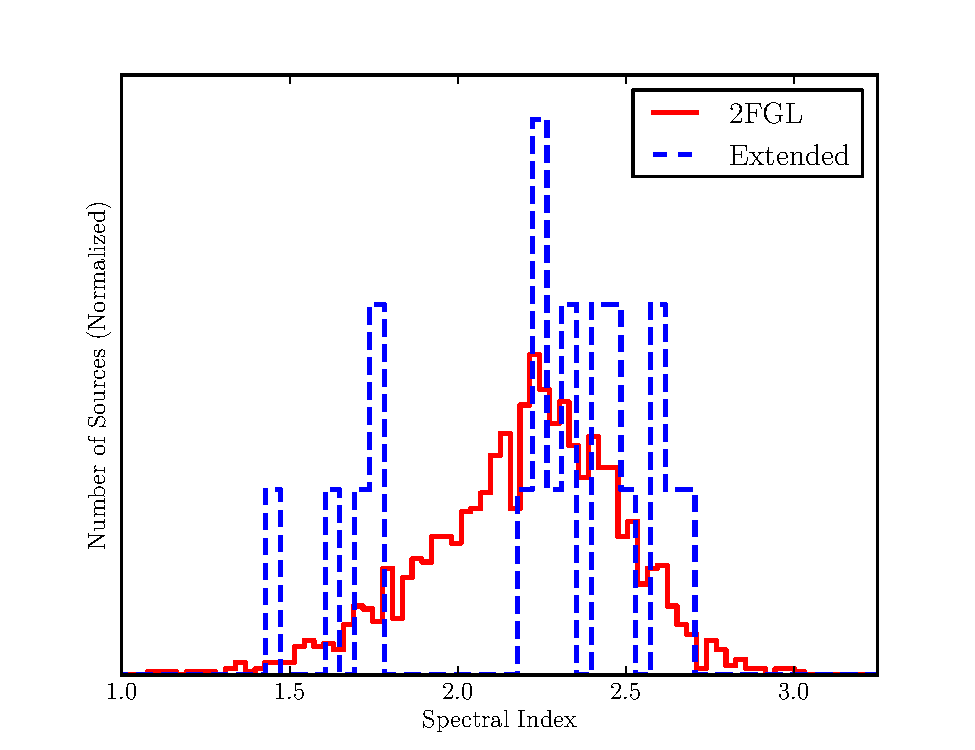
\includegraphics{summary_plots/compare_index_2FGL.pdf}
    % plot taken from /u/gl/lande/work/fermi/extended_catalog/2FGL/plots_for_paper/compare_index_2fgl/v3/run.py
    \end{center}
    \caption{
    The distribution of spectral indices of all 1873 2FGL sources in
    red and all spatially extended sources in blue.  in 2FGL. The
    spectral indices of LAT extended sources are taken from
    table~\ref{known_extended_sources} table~\ref{new_ext_srcs_table}.
    The index of Centarus A is taken to be 2.58 from the two year catalog
    (\cite{second_cat}) and the index of Vela X is taken to be 2.41
    from (\cite{velax}). This plot shows that many of the LAT
    extended sources have a hard ($<2$) spectral index.
    }\label{compare_index_2FGL}
  \end{figure}

  \clearpage
\begin{appendices}

\begin{figure}
  \begin{center}
    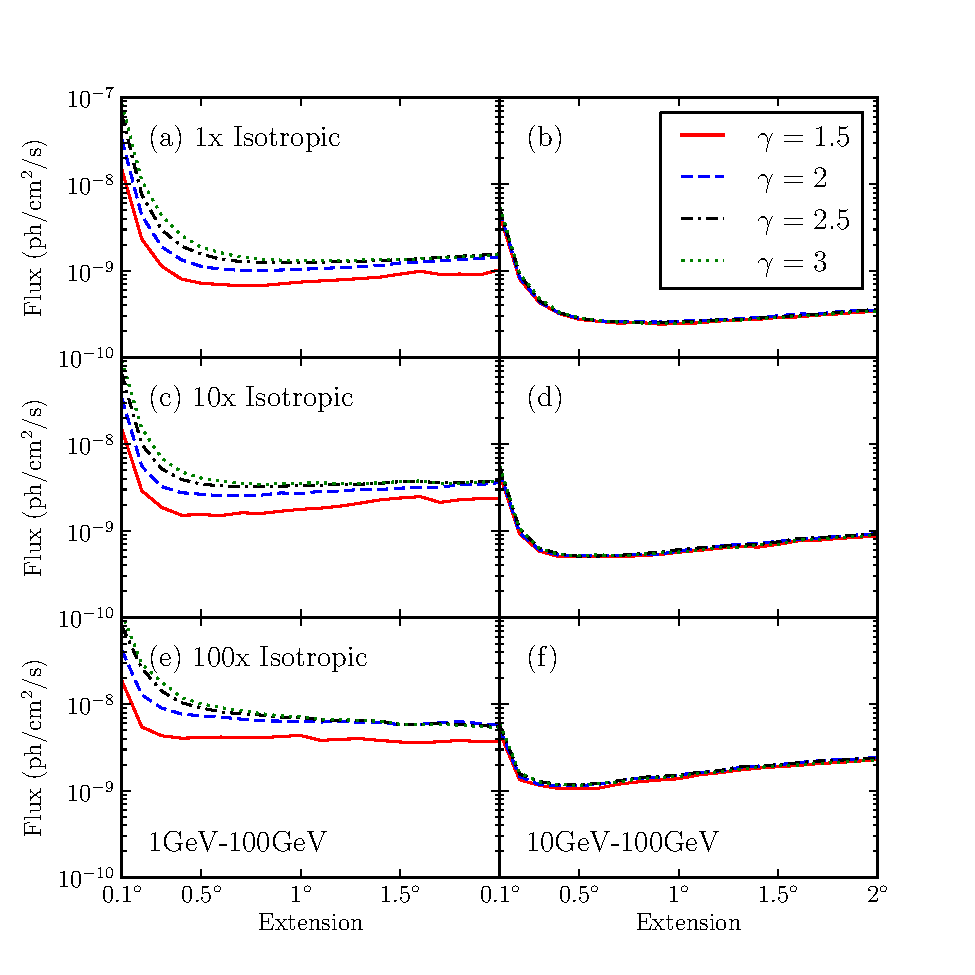
\includegraphics{mc_plots/all_sensitivity.pdf}
    % this plot came from /u/gl/lande/work/fermi/extended_catalog/monte_carlo/sensitivity/v12/plot/plot_all.py
    \end{center}
    \caption{These six plots condense the LAT detection threshold for
    all four spectral indices shown in figure~\ref{index_sensitivity}
    (1.5, 2, 2.5, and 3) and all three background levels shown
    in~\ref{diff_factor_sensitivity}.  (1x, 10x, and 100x the
    Sreekumar-like isotropic spectrum).  The plots have the same meaning
    as in figure~\ref{index_sensitivity} The left plots are the detection
    threshold when using the photons with energies between 1 \gev and
    100 \gev and the right plots are the detection threshold when using
    photons with energies between 10 \gev and 100 \gev.  This plot shows
    that when using only high energy photons with an improved angular
    resolution, our detection threshold is only weakly a function of
    spectral index. The numeric values plotted here are tabulated
    in table~\ref{all_sensitivity_table}. More information about this plot is presented
    in section~\ref{extension_sensitivity}.
    }\label{all_sensitivity} 
  \end{figure}

  \clearpage
  \thispagestyle{empty}
  \begin{sidewaystable}\scriptsize
    \begin{centering}
      \begin{tabular}{r|r|rrrrrrrrrrrrrrrrrrrr}
        \hline
        \hline
        \multicolumn{22}{c}{$ 1 \gev < E < 100 \gev$} \\
        \hline
        $\gamma$ &       BG &  $0.1\deg$ &  $0.2\deg$ &  $0.3\deg$ &  $0.4\deg$ &  $0.5\deg$ &  $0.6\deg$ &  $0.7\deg$ &  $0.8\deg$ &  $0.9\deg$ &    $1\deg$ &  $1.1\deg$ &  $1.2\deg$ &  $1.3\deg$ &  $1.4\deg$ &  $1.5\deg$ &  $1.6\deg$ &  $1.7\deg$ &  $1.8\deg$ &  $1.9\deg$ &    $2\deg$ \\
        \hline
             1.5 &       x1 &      149.5 &       23.5 &       11.4 &        8.1 &        7.2 &        7.0 &        6.8 &        6.8 &        7.0 &        7.4 &        7.5 &        7.7 &        7.9 &        8.2 &        8.9 &        9.7 &        9.0 &        9.0 &        8.7 &       10.1 \\
                 &      x10 &      145.7 &       28.9 &       18.3 &       15.1 &       15.4 &       15.0 &       16.1 &       15.8 &       16.6 &       17.6 &       18.5 &       19.9 &       21.5 &       23.6 &       25.2 &       25.2 &       21.4 &       23.0 &       23.6 &       23.8 \\
                 &     x100 &      184.2 &       55.3 &       42.1 &       40.6 &       40.5 &       42.0 &       42.1 &       40.6 &       43.0 &       43.7 &       37.6 &       39.4 &       39.9 &       36.8 &       35.9 &       36.1 &       36.3 &       37.7 &       37.0 &       37.4 \\
               2 &       x1 &      332.5 &       44.1 &       18.9 &       13.4 &       11.3 &       10.4 &       10.1 &       10.0 &       10.1 &       10.3 &       10.6 &       10.8 &       11.0 &       11.3 &       12.2 &       12.4 &       12.8 &       13.2 &       13.5 &       13.8 \\
                 &      x10 &      337.9 &       55.6 &       32.4 &       27.2 &       26.4 &       25.4 &       25.6 &       26.0 &       27.8 &       28.2 &       29.2 &       29.2 &       31.1 &       30.8 &       31.5 &       32.8 &       32.1 &       34.5 &       34.8 &       36.6 \\
                 &     x100 &      416.0 &      133.9 &       88.0 &       77.8 &       74.1 &       72.6 &       68.7 &       65.0 &       63.0 &       63.3 &       61.7 &       61.8 &       60.1 &       59.0 &       54.7 &       58.0 &       58.9 &       60.8 &       57.5 &       53.9 \\
             2.5 &       x1 &      635.5 &       74.3 &       29.8 &       19.2 &       15.8 &       13.7 &       12.8 &       12.7 &       12.3 &       12.4 &       12.4 &       12.6 &       12.7 &       12.9 &       13.3 &       13.4 &       13.8 &       14.3 &       14.7 &       15.4 \\
                 &      x10 &      640.0 &       97.6 &       51.7 &       39.3 &       34.6 &       33.0 &       32.7 &       32.6 &       33.0 &       33.5 &       34.6 &       35.2 &       34.7 &       36.0 &       37.3 &       37.3 &       35.7 &       36.4 &       37.5 &       38.1 \\
                 &     x100 &      794.9 &      261.2 &      134.2 &      103.5 &       89.5 &       80.7 &       78.1 &       75.3 &       70.1 &       70.2 &       65.5 &       64.7 &       61.9 &       59.8 &       56.4 &       55.6 &       57.9 &       55.0 &       53.3 &       51.8 \\
               3 &       x1 &      857.2 &      110.2 &       43.5 &       25.8 &       18.9 &       16.1 &       14.3 &       13.5 &       13.2 &       13.2 &       13.0 &       12.9 &       13.2 &       13.3 &       13.2 &       13.5 &       13.8 &       14.1 &       14.4 &       15.0 \\
                 &      x10 &      931.1 &      155.1 &       70.4 &       48.3 &       40.9 &       37.3 &       35.6 &       35.0 &       35.5 &       35.8 &       36.0 &       34.9 &       35.1 &       35.1 &       37.0 &       37.7 &       35.4 &       35.8 &       36.6 &       37.8 \\
                 &     x100 &     1119.8 &      295.6 &      180.9 &      119.4 &      101.0 &       92.0 &       86.4 &       78.5 &       73.5 &       69.9 &       66.7 &       64.9 &       63.3 &       61.2 &       57.3 &       56.7 &       56.7 &       55.0 &       50.7 &       50.4 \\
        \hline
        \multicolumn{22}{}{} \\
        \multicolumn{22}{}{} \\
        \hline
        \hline
        \multicolumn{22}{c}{$ 10 \gev < E < 100 \gev$} \\
        \hline
        $\gamma$ &       BG &  $0.1\deg$ &  $0.2\deg$ &  $0.3\deg$ &  $0.4\deg$ &  $0.5\deg$ &  $0.6\deg$ &  $0.7\deg$ &  $0.8\deg$ &  $0.9\deg$ &    $1\deg$ &  $1.1\deg$ &  $1.2\deg$ &  $1.3\deg$ &  $1.4\deg$ &  $1.5\deg$ &  $1.6\deg$ &  $1.7\deg$ &  $1.8\deg$ &  $1.9\deg$ &    $2\deg$ \\
        \hline
             1.5 &       x1 &       43.9 &        8.2 &        4.3 &        3.2 &        2.8 &        2.6 &        2.6 &        2.6 &        2.6 &        2.6 &        2.6 &        2.7 &        2.8 &        2.8 &        3.0 &        3.0 &        3.1 &        3.3 &        3.4 &        3.5 \\
                 &      x10 &       44.6 &        9.1 &        5.8 &        5.0 &        5.0 &        5.1 &        5.0 &        5.4 &        5.3 &        5.7 &        6.0 &        6.3 &        6.7 &        6.5 &        7.1 &        7.7 &        7.8 &        8.2 &        8.4 &        8.7 \\
                 &     x100 &       47.2 &       13.3 &       11.4 &       10.6 &       10.6 &       10.7 &       11.9 &       12.7 &       13.2 &       13.6 &       15.3 &       16.2 &       17.4 &       18.4 &       19.3 &       20.1 &       20.8 &       21.8 &       22.6 &       24.0 \\
               2 &       x1 &       49.1 &        8.5 &        4.4 &        3.3 &        2.8 &        2.7 &        2.7 &        2.7 &        2.7 &        2.7 &        2.7 &        2.8 &        2.9 &        3.0 &        3.1 &        3.2 &        3.2 &        3.4 &        3.5 &        3.6 \\
                 &      x10 &       48.3 &        9.6 &        6.0 &        5.2 &        5.2 &        5.3 &        5.3 &        5.6 &        5.5 &        5.9 &        6.4 &        6.7 &        7.0 &        7.2 &        7.7 &        8.0 &        8.3 &        8.6 &        9.0 &        9.3 \\
                 &     x100 &       51.1 &       14.8 &       11.7 &       11.4 &       11.5 &       12.0 &       13.1 &       14.0 &       14.4 &       15.2 &       16.1 &       17.1 &       18.7 &       19.7 &       20.5 &       21.9 &       22.9 &       23.7 &       24.1 &       25.2 \\
             2.5 &       x1 &       52.1 &        9.2 &        4.6 &        3.3 &        2.9 &        2.7 &        2.7 &        2.7 &        2.7 &        2.7 &        2.7 &        2.8 &        2.9 &        2.9 &        3.0 &        3.1 &        3.2 &        3.4 &        3.4 &        3.6 \\
                 &      x10 &       53.0 &       10.5 &        6.2 &        5.4 &        5.2 &        5.2 &        5.4 &        5.6 &        5.8 &        6.1 &        6.4 &        6.6 &        6.9 &        7.3 &        7.5 &        8.2 &        8.4 &        8.7 &        8.9 &        9.3 \\
                 &     x100 &       55.5 &       15.9 &       12.7 &       12.0 &       11.9 &       12.3 &       13.0 &       14.4 &       14.7 &       15.2 &       16.4 &       17.2 &       19.1 &       19.6 &       20.6 &       21.9 &       23.0 &       23.4 &       24.4 &       24.9 \\
               3 &       x1 &       54.6 &        9.5 &        4.7 &        3.4 &        2.9 &        2.7 &        2.6 &        2.5 &        2.5 &        2.6 &        2.6 &        2.7 &        2.7 &        2.9 &        2.9 &        3.0 &        3.1 &        3.2 &        3.4 &        3.4 \\
                 &      x10 &       55.1 &       10.5 &        6.2 &        5.3 &        5.2 &        5.3 &        5.2 &        5.4 &        5.5 &        5.7 &        6.0 &        6.4 &        6.6 &        7.0 &        7.3 &        7.9 &        8.1 &        8.5 &        8.7 &        8.9 \\
                 &     x100 &       59.8 &       16.0 &       12.7 &       11.8 &       11.6 &       12.2 &       12.7 &       14.1 &       14.2 &       14.6 &       16.0 &       16.9 &       17.9 &       19.0 &       20.1 &       20.6 &       21.6 &       22.1 &       22.7 &       23.5 \\
        \hline
      \end{tabular}
      \caption{The detection threshold to resolve a uniform disk spatially
      extended sources using two years of data for sources of varying
      spectral index and extension against varying background levels
      with different energy ranges.  The upper table is the sensitivity
      when using photons with energies from 1-100 \gev and the bottom
      table is when using 10-100 \gev photons. The first column is
      the extended source's spectral index.  The extended sources
      were simulated against a Sreekumar-like isotropic spectrum and
      the second column is the factor that the simulated background
      was scaled by. The remaining columns are varying sizes of the
      source's spatial model. The table quotes fluxes in units of
      $10^{-10} \ph/\cm^2/\sec$.  These values are also plotted in
      figure~\ref{all_sensitivity}.  More information about this
      table is presented in section~\ref{extension_sensitivity}.
      }\label{all_sensitivity_table}
    \end{centering}
  \end{sidewaystable}

\end{appendices}

\end{document}
